\documentclass[12pt]{article} 
\usepackage[T1]{fontenc} 
\usepackage[utf8]{inputenc} 
\usepackage[serbian]{babel} 
\usepackage{lmodern} 
\usepackage[expansion=false]{microtype} 
\usepackage{amsmath, amsthm, amssymb} 
\usepackage{graphicx} 
\usepackage{subfigure} % za \subfigure komandu 
\usepackage{tikz} 
\usepackage{dblfloatfix} 
\usepackage{tabto} 
\usepackage{float} 
\usepackage{booktabs} 
\usepackage{multirow} 
\usepackage{tabularx} 
\usepackage{newtxtext}
\usepackage{hyperref}

\usepackage[a4paper, left=2cm, right=2cm, top=2.5cm, bottom=2.5cm]{geometry}
%\usepackage{hyperref} % UVEK zadnji 
\renewcommand{\baselinestretch}{1.0} 
% \newtheorem{pri}{Пример}[subsection] 
% \newtheorem{defi}{Дефиниција}[subsection] 
% \newtheorem{teo}{Теорема}[subsection] 
\usepackage{enumitem}  

% \newtheorem{lemma}{Лема}[subsection]

% \newtheorem{innercustomthm}{Задатак}
% \newenvironment{customthm}[1]
  
% \newtheorem{seq}{Последица}[subsection]
\renewcommand\qedsymbol{$\blacksquare$}
\def\contentsname{Sadržaj}
\def\chaptername{Glava}
\def\bibname{Literatura}
\def\tablename{Tabela}
\def\figurename{Slika}
\def\appendixname{Dodatak}
\renewcommand{\refname}{Literatura}
\usepackage[nottoc]{tocbibind}

\setcounter{page}{1}
\title{Modelovanje i predikcija koncentracija polena u Srbiji korišćenjem geostatistike i mašinskog učenja}
\author{Luka Milutinović}
\date{Univerzitet u Beogradu, Elektrotehnički fakultet, 2025.}
\begin{document}
\newpage

\begin{figure}[H]
    \centering
    \includegraphics[width=2cm]{grafici/etflogotip.png}

\end{figure}

\begin{center}
\large \textbf{UNIVERZITET U BEOGRADU}
\end{center}
\begin{center}
\large \textbf{ELEKTROTEHNIČKI FAKULTET}
\end{center}



\thispagestyle{empty}


\vspace*{3cm}
\begin{center}
\Huge \textbf{Modelovanje i predikcija koncentracija polena u Srbiji korišćenjem geostatistike i mašinskog učenja}
\end{center}


\begin{center}
\small \textbf{DIPLOMSKI RAD}
\end{center}


\vspace*{6cm}

\begin{center}

\begin{tabular}{ccc}
\large Student & \hspace*{3cm} & \large Mentor \\
 & & \\
\large\textbf{Luka Milutinović} & & \large\textbf{} \\
\large\textsl{2021/0103} & & \large\textsl{} \\

\end{tabular}
\end{center}

\vspace*{0.9cm}

\begin{center}
\normalsize	 BEOGRAD,  2025.
\end{center}

\mbox{}
\newpage
\thispagestyle{empty}
\tableofcontents
\thispagestyle{empty}
\mbox{}
\newpage

\section{Uvod}
\setcounter{page}{1}
\hspace*{\parindent}
U poslednjih nekoliko decenija, sve veća pažnja posvećuje se praćenju koncentracije polena u vazduhu zbog njegovog značajnog uticaja na zdravlje ljudi i svakodnevni život. Polen je jedan od glavnih alergena u spoljašnjoj sredini, pa osobe koje pate od polenskih alergija često osećaju pogoršanje simptoma upravo u vreme cvetanja biljaka. Tačna i pravovremena prognoza koncentracije polena može da bude ključna za blagovremeno započinjanje terapije, što pomaže u smanjenju jačine i trajanja neprijatnih simptoma.

Zbog urbanizacije, zagađenja vazduha i klimatskih promena, broj osoba koje pate od polenskih alergija u stalnom je porastu širom sveta, pa i u Srbiji. Prema dostupnim podacima, procenjuje se da između 30\% i 40\% stanovništva Srbije ima neku formu alergije na polen \cite{bionette2023, drugacijipristup2025}.

Klinička istraživanja su pokazala da osobe koje započnu terapiju protiv polenske alergije nedelju dana pre početka sezone imaju značajno blaže simptome u poređenju sa onima koji terapiju započinju tek kada simptomi nastupe, što naglašava značaj lokalno precizne prognoze polena za planiranje terapije i smanjenje zdravstvenih problema \cite{omalizumab2022, birch2019}.

Predviđanje koncentracije polena predstavlja složen zadatak, jer zavisi od sezonskih obrazaca, meteoroloških faktora (temperatura, vetar, padavine, vlažnost), kao i od učestalog problema nedostajućih podataka. Proces merenja zahteva kontinuirano praćenje i laboratorijsku analizu, što se zbog tehničkih i finansijskih ograničenja često ne sprovodi u kontinuitetu, pa podaci ostaju nepotpuni ili nedostupni u određenim vremenskim i prostornim intervalima \cite{minic2020, sofia2023}.

Da bi se rešio problem nedostajućih vrednosti i omogućilo pouzdano predviđanje, u ovom radu je korišćena metoda \textit{spatio-temporal kriging}-a za popunjavanje podataka. Nakon toga, za predikciju koncentracije polena primenjeni su modeli vremenskih serija i mašinskog učenja: \textbf{SARIMAX}, \textbf{Prophet} i \textbf{Random Forest} regresija.

\subsection{Cilj rada}
Cilj ovog rada je da se razvije i implementira sistem za predikciju koncentracije polena korišćenjem modela vremenskih serija i mašinskog učenja, uz prethodnu imputaciju nedostajućih vrednosti pomoću geostatističkih metoda, kako bi se unapredila tačnost i pouzdanost prognoze, a time i omogućila pravovremena reakcija osoba sa alergijama, unapređenje pčelarske proizvodnje i doprinosi uspešnijem oprašivanju biljaka u poljoprivredi.

\subsection{Struktura rada}
Prvo poglavlje predstavlja uvod i motivaciju za istraživanje. Drugo poglavlje daje teorijski osnov o polenu, modelima vremenskih serija, mašinskom učenju i geostatistici. Treće poglavlje opisuje materijale i metode, uključujući opis podataka, predprocesiranje, imputaciju i treniranje modela. Četvrto poglavlje prikazuje rezultate eksperimenta i diskusiju o dobijenim rezultatima. Peto poglavlje donosi zaključke i predloge za budući rad.
\newpage
\section{Teorijski osnov}

\subsection{Polen i alergije}
Polen su mikroskopske čestice koje biljke proizvode tokom reprodukcije, a njihov osnovni biološki zadatak je oprašivanje \cite{pollenBio2021}. U vazduhu se najčešće nalaze poleni drveća, trava i korova, posebno oni koje vetar lako prenosi na velike udaljenosti \cite{sofia2023}. Veličina polenovih zrna varira od 10 do 100 mikrometara, što im omogućava da se lako šire i dugo zadrže u atmosferi \cite{piotrowska2012}.

Svaka biljna vrsta proizvodi svoj karakteristični polen, a dominantni tipovi polena u vazduhu menjaju se tokom godine. U proleće preovlađuju poleni drveća poput breze, leske i jove, u kasno proleće i početkom leta dominiraju poleni trava, dok krajem leta i početkom jeseni dominira polen korova poput ambrozije \cite{birch2019}. Najčešće alergijske reakcije izazivaju poleni trava, ambrozije i drveća, a posebno je problematična ambrozija zbog dugog perioda cvetanja i visoke koncentracije polena, zbog čega predstavlja jedan od najzastupljenijih i najjačih alergena u regionu \cite{omalizumab2022}.

Alergijska reakcija nastaje kada imuni sistem prepozna polen kao stranu i potencijalno opasnu supstancu, iako on sam po sebi nije štetan \cite{bionette2023}. Tipični simptomi uključuju svrab očiju i nosa, kijanje, curenje nosa, suzenje očiju, dok kod osoba sa astmom može doći do otežanog disanja i napada gušenja. Ovi simptomi često dovode do problema sa spavanjem, osećaja hroničnog umora i smanjene koncentracije, što značajno utiče na svakodnevnu produktivnost \cite{minic2020}. Istraživanja pokazuju da alergijski rinitis može dovesti do smanjenja radne efikasnosti i do 40\%, posebno u periodima visoke koncentracije polena \cite{sofia2023}.
Ipak, polen ima i korisne aspekte. Za pčelarstvo je od presudne važnosti jer predstavlja glavni izvor proteina za pčele, neophodan za razvoj legla i jačanje pčelinjeg društva, čime se direktno utiče na proizvodnju meda i polena kao dijetetskog suplementa \cite{pollenBio2021}. U poljoprivredi obezbeđuje oprašivanje, ključno za stabilne i visoke prinose mnogih kultura, dok se u ekologiji i palinologiji koristi za proučavanje promena vegetacije i klime tokom istorije, budući da polen ostaje sačuvan u sedimentima hiljadama godina \cite{piotrowska2012}.

Koncentracija polena u vazduhu zavisi od vrste biljaka, geografskog područja, kao i od meteoroloških faktora poput temperature, padavina, vlažnosti i brzine vetra \cite{chico2025}. Ovi faktori zajedno određuju vreme i intenzitet oslobađanja polena, zbog čega predikcija koncentracije polena zahteva modele koji uzimaju u obzir sezonske obrasce i promene u okruženju \cite{sofia2023}. Razumevanje i predviđanje dinamike polena u vazduhu od velikog su značaja za javno zdravlje, pčelarstvo, poljoprivredu i ekološka istraživanja \cite{minic2020}.

\subsection{Uvod i značaj vremenskih serija}
Predviđanje budućih događaja oduvek je fasciniralo čovečanstvo. Još od najranijih vremena ljudi su posmatrali kretanje zvezda, Mesečeve mene i promene godišnjih doba kako bi znali kada da seju, žanju ili migriraju. Danas se predviđanje temelji na matematičkim i statističkim metodama, ali osnovna ideja ostaje nepromenjena – težnja ka sagledavanju i razumevanju budućih pojava i procesa. Na primer, stari Egipćani su pre više od 4000 godina beležili nivo reke Nil kako bi procenili plodnost zemljišta i planirali raspodelu resursa. Time su, iako nesvesno, primenjivali principe vremenskih serija, iako tada nije postojao formalni statistički okvir kakav danas poznajemo \cite{metnil2025}.

Kroz istoriju, međutim, predviđanje nije uvek bilo prihvaćeno. U starom Rimu, car Konstantin II je 357. godine nove ere izdao dekret kojim je zabranio svako proricanje budućnosti i konsultovanje matematičara ili astrologa, smatrajući da takve aktivnosti mogu ugroziti vlast i izazvati nemire. Slično tome, u Engleskoj je 1824. godine donet zakon prema kojem su svi koji su tvrdili da mogu da predviđaju budućnost proglašavani za prevarante i osuđivani na zatvor i prinudni rad. Iako su ove zabrane bile usmerene na astrologiju i gatanje, one pokazuju da je pokušaj predikcije kroz istoriju imao i snažnu društvenu i političku težinu \cite{histlaw2025}.

Prvi značajni matematički radovi o vremenskim serijama pojavili su se početkom 20. veka, kada su \textit{Yule} i \textit{Slutsky} postavili temelje teorije linearnih modela, uvodeći ključne pojmove poput autoregresivnih procesa i analize periodičnih komponenti ekonomskih podataka \cite{yule1927, slutsky1937}. Tokom 1950-ih i 1960-ih, \textit{Robert G. Brown} je popularizovao metodu eksponencijalnog zaglađivanja, omogućivši jednostavna i efikasna predviđanja u industrijskoj praksi. Dalje, 1970. godine, \textit{Box} i \textit{Jenkins} razvili su \textbf{ARIMA} metodologiju, čime su otvorili put za praktičnu i sistematsku primenu analiza vremenskih serija u ekonomiji, inženjerstvu i brojnim drugim oblastima \cite{box1970}.

Danas se vremenske serije definišu kao niz uzastopnih posmatranja neke promenljive ${Y_t}$ prikupljenih kroz vreme, gde je redosled posmatranja od suštinskog značaja.

\subsubsection{Primeri primene}
\begin{itemize}
    \item U meteorologiji, vremenske serije se koriste za prognozu temperature, padavina i vetra, što direktno utiče na planiranje u poljoprivredi.
    \item U finansijama, primenjuju se za analizu i predikciju cena akcija, deviznih kurseva i tržišnih indeksa.
    \item U energetici, omogućavaju planiranje proizvodnje i balansiranje potrošnje električne energije.
    \item U biomedicini, koriste se za analizu srčanog ritma, EEG i drugih fizioloških signala radi dijagnostike i praćenja stanja pacijenata.
\end{itemize}
\subsubsection{Matematičko definisanje i komponente vremenskih serija}

Vremenska serija predstavlja realizaciju stohastičkog procesa čije se vrednosti posmatraju u različitim vremenskim tačkama \cite{yule1927, box1970}. Formalno, vremenska serija je skup slučajnih promenljivih:

\[
\{Y_t\}, \quad t \in T
\]

gde je $T$ diskretan skup vremena, a $Y_t$ realizacija promenljive u trenutku $t$.

U praktičnoj analizi vremenskih serija, radimo sa jednom realizacijom i pretpostavljamo da ona odražava svojstva celog stohastičkog procesa \cite{slutsky1937}.

Svaka vremenska serija može se razložiti na nekoliko komponenti koje zajedno definišu njeno ponašanje. Te komponente su:

\begin{itemize}
    \item \textbf{Trend ($T_t$)}: dugoročna promena u nivou serije kroz vreme. Može biti rastući, opadajući ili stabilan.
    
    \item \textbf{Sezonalnost ($S_t$)}: obrazac koji se ponavlja u pravilnim vremenskim intervalima, npr. godišnja sezonalnost koncentracije polena \cite{sofia2023}.
    
    \item \textbf{Cikličnost ($C_t$)}: oscilacije koje se javljaju u nepravilnim i dužim vremenskim intervalima, često povezane sa ekonomskim ciklusima ili klimatskim promenama.
    
    \item \textbf{Slučajna komponenta ($R_t$)}: reziduali koji se ne mogu objasniti trendom, sezonalnošću ili cikličnošću; predstavljaju šum u podacima.
\end{itemize}

Postoje dva osnovna modela dekompozicije vremenskih serija \cite{yule1927, box1970}:

\begin{itemize}
    \item \textbf{Aditivni model}:
    \begin{equation*}
        Y_t = T_t + S_t + C_t + R_t
    \end{equation*}
    Koristi se kada su amplitude sezonalnosti i fluktuacija nezavisne od nivoa serije.
    
    \item \textbf{Multiplikativni model}:
    \begin{equation*}
        Y_t = T_t \times S_t \times C_t \times R_t
    \end{equation*}
    Koristi se kada amplitude sezonalnosti i šuma rastu proporcionalno nivou serije.
\end{itemize}



\noindent



\subsubsection{Stacionarnost i testovi stacionarnosti (ADF i KPSS)}
\label{sec:stationarity}
Za većinu metoda analize vremenskih serija, posebno za \textbf{ARIMA} modele, stacionarnost je osnovna pretpostavka za statistički validno i pouzdano modeliranje \cite{box1970, dickey1979, kpss1992}. U praktičnom smislu, stacionarna serija ima:

\begin{itemize}
    \item konstantnu srednju vrednost
    \item konstantnu varijansu kroz vreme
    \item kovarijansu koja zavisi samo od vremenskog pomaka, a ne od samog vremena.
\end{itemize}

Formalno, vremenska serija $\{Y_t\}$ je slabo stacionarna ako:

\begin{equation*}
E[Y_t] = \mu
\end{equation*}
\begin{equation*}
Var(Y_t) = \sigma^2
\end{equation*}
\begin{equation*}
Cov(Y_t, Y_{t+h}) = \gamma(h)
\end{equation*}

\noindent gde su $\mu$ i $\sigma^2$ konstante, a $\gamma(h)$ zavisi samo od vremenskog pomaka $h$, a ne od samog vremena $t$ \cite{box1970}.

\bigskip

\noindent Serija je strogo stacionarna ako zajednička raspodela bilo kog vektora
\[
F_X(Y_{t_1}, Y_{t_2}, ..., Y_{t_k})
\]
ostaje nepromenjena za svaki vremenski pomak $h$, odnosno:
\[
F_X(Y_{t_1}, Y_{t_2}, ..., Y_{t_k}) = F_X(Y_{t_1 + h}, Y_{t_2 + h}, ..., Y_{t_k + h})
\]
za svako $k$ i $h$ \cite{box1970}.

U praksi, uslov striktne stacionarnosti je veoma jak i teško proverljiv, te se za većinu modela koristi slaba stacionarnost, koja zahteva konstantnu sredinu, konstantnu varijansu i kovarijansu koja zavisi samo od vremenskog pomaka \cite{dickey1979, kpss1992}.
\paragraph{Augmented Dickey-Fuller (ADF) test}

\noindent Jedan od najčešće korišćenih testova za proveru stacionarnosti vremenskih serija je \textbf{Augmented Dickey-Fuller (ADF) test} \cite{dickey1979, box1970}. Ovaj test se primarno koristi za ispitivanje prisustva \textbf{jediničnog korena (unit root)} u vremenskoj seriji.

\bigskip

\noindent \textbf{Jedinični koren.} Vremenska serija poseduje jedinični koren ako sadrži komponentu slučajnog hoda, što implicira nestacionarnost. Na primer, AR(1) proces definisan kao:
\[
Y_t = \phi Y_{t-1} + \epsilon_t,
\]
gde je $\epsilon_t$ beli šum, biće stacionaran ako $|\phi| < 1$. Kada $\phi = 1$, model prelazi u formu slučajnog hoda:

\[
Y_t = Y_{t-1} + \epsilon_t,
\]
kod koje varijansa raste linearno kroz vreme, što znači da proces nije stacionaran.


\noindent \textbf{Izvod regresione forme ADF testa.}

Osnovni \textit{Dickey-Fuller} test polazi od AR(1) modela:

\[
Y_t = \phi Y_{t-1} + \epsilon_t.
\]

Oduzimanjem $Y_{t-1}$ sa obe strane, dobija se:

\[
Y_t - Y_{t-1} = \phi Y_{t-1} - Y_{t-1} + \epsilon_t,
\]

\[
\Delta Y_t = (\phi - 1) Y_{t-1} + \epsilon_t.
\]

Neka je $\gamma = \phi - 1$, dobija se osnovni oblik regresione jednačine:

\[
\Delta Y_t = \gamma Y_{t-1} + \epsilon_t.
\]

\noindent Testiranje hipoteze $\phi = 1$ ekvivalentno je testiranju $\gamma = 0$.


\noindent \textbf{Augmented Dickey-Fuller (ADF) regresioni model.}

ADF test proširuje osnovni \textit{Dickey-Fuller} test uključivanjem:

\begin{itemize}
    \item konstantnog člana ($\alpha$),
    \item determinističkog trenda ($\beta t$),
    \item i $p$ zaostalih diferenciranih vrednosti $\Delta Y_{t-i}$ radi eliminacije autokorelacije u rezidualima.
\end{itemize}

\noindent Konačna regresiona forma ADF testa glasi:

\[
\Delta Y_t = \alpha + \beta t + \gamma Y_{t-1}
+ \sum_{i=1}^{p} \delta_i \Delta Y_{t-i}
+ \epsilon_t.
\]


\noindent \textbf{Hipoteze ADF testa:}

\begin{itemize}
\item $H_0$: serija ima jedinični koren (nije stacionarna), tj. $\gamma = 0$,
\item $H_1$: serija je stacionarna, tj. $\gamma \neq 0$.
\end{itemize}

\noindent Odluka se donosi na osnovu procene parametra $\gamma$. Ako je $\gamma$ značajno manji od nule, odbacuje se nulta hipoteza i zaključuje da je serija stacionarna. Kritične vrednosti za ADF test razlikuju se od standardnih vrednosti t-raspodele i određene su tablično.

\paragraph{KPSS (Kwiatkowski-Phillips-Schmidt-Shin) test}

\noindent \textbf{KPSS test} je statistički test koji se koristi za proveru stacionarnosti vremenskih serija \cite{kpss1992}. Za razliku od ADF testa, KPSS test ima \textbf{suprotne hipoteze}.

\bigskip
\noindent \textbf{Hipoteze KPSS testa:}
\begin{itemize}
    \item $H_0$: vremenska serija je stacionarna (oko konstante ili determinističkog trenda),
    \item $H_1$: vremenska serija nije stacionarna (ima jedinični koren).
\end{itemize}

\noindent \textbf{Model KPSS testa.}
KPSS test polazi od modela vremenske serije zapisanog kao:
\[
Y_t = r_t + \beta t + \epsilon_t,
\]
gde je:
\begin{itemize}
    \item $r_t$ – komponenta slučajnog hoda,
    \item $\beta t$ – deterministički trend,
    \item $\epsilon_t$ – stacionarna greška (beli šum).
\end{itemize}

\noindent Komponenta slučajnog hoda definiše se kao:
\[
r_t = r_{t-1} + u_t,
\]
gde je $u_t$ beli šum. Ako je varijansa $u_t$ jednaka nuli, tada je $r_t$ konstantan i $Y_t$ je trend-stacionaran \cite{kpss1992}.

\bigskip

\noindent \textbf{Interpretacija rezultata.}

KPSS test ispituje prisustvo komponente slučajnog hoda u vremenskoj seriji:

\begin{itemize}
    \item Ako komponenta slučajnog hoda \textit{ne postoji} ($var(u_t)=0$), serija je stacionarna oko konstante ili trenda.
    \item Ako komponenta slučajnog hoda \textit{postoji} ($var(u_t)>0$), serija je nestacionarna jer varijansa raste kroz vreme.
\end{itemize}

\bigskip

\noindent \textbf{Test statistika.}

KPSS test statistika se računa kao:
\[
KPSS = \frac{1}{T^2} \sum_{t=1}^{T} S_t^2 / \hat{\sigma}^2,
\]
gde je:
\begin{itemize}
    \item $S_t$ – kumulativna suma reziduala, $S_t = \sum_{i=1}^{t} e_i$,
    \item $\hat{\sigma}^2$ – procena dugoročne varijanse reziduala,
    \item $T$ – veličina uzorka.
\end{itemize}

\noindent Ako je vrednost test statistike veća od kritične vrednosti, odbacuje se nulta hipoteza i zaključuje da serija nije stacionarna \cite{kpss1992}.

\bigskip

\noindent \textbf{Kombinacija sa ADF testom.}

U praksi se preporučuje upotreba KPSS testa zajedno sa ADF testom, jer imaju suprotne hipoteze:

\begin{itemize}
    \item Ako ADF odbacuje $H_0$ (serija je stacionarna) i KPSS ne odbacuje $H_0$ (serija je stacionarna), zaključuje se stacionarnost.
    \item Ako ADF ne odbacuje $H_0$ (serija nije stacionarna) i KPSS odbacuje $H_0$ (serija nije stacionarna), zaključuje se nestacionarnost.
    \item Ako su rezultati kontradiktorni, potrebna je dodatna analiza (diferenciranje, transformacije, vizuelna analiza) \cite{dickey1979, kpss1992}.
\end{itemize}

\subsubsection{Box-Cox transformacija}

\textbf{Box-Cox transformacija} predstavlja metodu koja primenjuje različite funkcionalne oblike na podatke s ciljem stabilizacije varijanse i približavanja raspodele normalnoj \cite{boxcox1964}.

\bigskip

Transformacija se definiše na sledeći način:

$$
Y_t^{(\lambda)} =
\begin{cases}
\frac{Y_t^{\lambda} - 1}{\lambda}, & \lambda \neq 0 \\[6pt]
\ln(Y_t), & \lambda = 0
\end{cases}
$$

gde je $Y_t$ posmatrana vrednost vremenske serije.

\bigskip

Parametar $\lambda$ određuje oblik transformacione funkcije i bira se tako da maksimizuje verodostojnost modela, omogućavajući da transformisani podaci što bolje prate normalnu raspodelu.

\bigskip

\textit{Box-Cox} transformacija ima dva osnovna cilja:

\begin{enumerate}
\item \textbf{Stabilizacija varijanse.}

Kod mnogih vremenskih serija varijansa zavisi od nivoa serije (heteroskedastičnost). Primena ove transformacije omogućava da varijansa bude približno konstantna bez obzira na nivo, što je ključno za korišćenje linearnih modela poput \textbf{ARIMA} i \textbf{SARIMAX}.

\item \textbf{Približavanje normalnosti raspodele.}

Brojne statističke metode pretpostavljaju normalno distribuirane greške. \textit{Box-Cox} transformacija omogućava da distribucija podataka bude bliža normalnoj, čime se poboljšava tačnost procene parametara i predikcija modela.
\end{enumerate}

\subsubsection{Beli šum}

\textbf{Beli šum} predstavlja osnovni koncept u teoriji vremenskih serija i stohastičkih procesa \cite{box1970, brockwell2002}. Formalno, beli šum je sekvenca nezavisnih i identično distribuiranih slučajnih promenljivih sa konstantnim očekivanjem i varijancom.

Matematički, niz $\epsilon_t$ predstavlja beli šum ako:

$$
E[\epsilon_t] = 0,
$$
$$
Var(\epsilon_t) = \sigma^2,
$$
$$
Cov(\epsilon_t, \epsilon_{t+\tau}) = 0, \quad \text{za svaki } \tau \neq 0.
$$

Karakteristike belog šuma:

\begin{itemize}
\item Vrednosti su statistički među sobom nezavisne.
\item Vrednosti imaju istu varijansu.
\item Nema serijske autokorelacije – koeficijent autokorelacije jednak je nuli za sve vremenske pomake osim za lag $t=0$.
\item Spektralna gustina je konstantna, što znači da su sve frekvencije podjednako zastupljene, analogno „belom svetlu“ koje sadrži sve talasne dužine.
\end{itemize}

Beli šum ima ključnu ulogu u modeliranju vremenskih serija jer predstavlja osnovnu pretpostavku za reziduale – nakon uklanjanja trenda, sezonalnosti i cikličnih komponenti, reziduali bi trebalo da se ponašaju kao beli šum. Analiza njihove autokorelacije koristi se za proveru adekvatnosti modela; ako reziduali nisu beli šum, to ukazuje da model nije obuhvatio sve obrasce u podacima i potrebno ga je unaprediti \cite{box1970, brockwell2002}.


\subsubsection{Autokorelacija (ACF) i parcijalna autokorelacija (PACF)}

Autokorelacija predstavlja meru povezanosti između posmatranja vremenske serije koja su međusobno udaljena za $k$ vremenskih jedinica (lag) \cite{box1970, brockwell2002}. Formalno, autokorelacija reda $k$ definiše se kao:

\[
\rho_k = \frac{Cov(Y_t, Y_{t-k})}{Var(Y_t)}.
\]

Autokorelaciona funkcija (ACF) prikazuje autokorelacije za sve vrednosti kašnjenja $k$, pri čemu za slabostacionarne procese važi:

\begin{itemize}
    \item $\rho_0 = 1$,
    \item $|\rho_k| < \rho_0, \quad \text{za } k>0$,
    \item $\lim_{k \to \infty} \rho_k = 0$.
\end{itemize}

\bigskip

\noindent \textbf{Intervali poverenja za ACF}

Za stacionarnu seriju bez autokorelacije (beli šum), standardna greška (SE) procene autokorelacije reda $k$ aproksimira se kao:

\[
SE(\rho_k) \approx \frac{1}{\sqrt{N}},
\]

gde je $N$ broj posmatranja. Za 95\% interval poverenja koristi se aproksimacija:

\[
\pm \frac{1.96}{\sqrt{N}}.
\]

Preciznija formula (Box-Jenkins) uzima u obzir prethodne autokorelacije:

\[
SE(\rho_k) = \sqrt{\frac{1 + 2 \sum_{i=1}^{k-1} \rho_i^2}{N}}.
\]

\bigskip

\noindent \textbf{Parcijalna autokorelacija (PACF)}

Parcijalna autokorelacija meri povezanost između $Y_t$ i $Y_{t-k}$ nakon što se eliminiše uticaj svih posrednih vrednosti između njih \cite{brockwell2002, hamilton1994}. PACF reda $k$ definiše se kao poslednji koeficijent $\phi_{kk}$ u AR($k$) modelu:

\[
Y_t = \phi_{k1} Y_{t-1}
     + \phi_{k2} Y_{t-2}
     + \cdots
     + \phi_{kk} Y_{t-k}
     + \epsilon_t.
\]

Intuitivno:

\begin{itemize}
    \item $\phi_{kk}$ predstavlja direktnu (parcijalnu) korelaciju između $Y_t$ i $Y_{t-k}$ uz eliminaciju uticaja svih kašnjenja između.
    \item Prethodni koeficijenti $\phi_{k1}, \ldots, \phi_{k(k-1)}$ uklanjaju indirektne veze preko bližih lagova.
\end{itemize}

\bigskip

\noindent \textbf{Računanje PACF}

PACF se računa pomoću:

\begin{enumerate}
    \item \textit{Yule-Walker} jednačina (rekurzivno) \cite{brockwell2002},
    \item Regresionih metoda, gde se za svaki lag $k$ fituje AR($k$) model, a PACF reda $k$ je poslednji koeficijent $\phi_{kk}$.
\end{enumerate}

\bigskip

\noindent \textbf{Intervali poverenja za PACF}

Pod pretpostavkom belog šuma, standardna greška PACF približno je jednaka standardnoj grešci ACF:

\[
SE \approx \frac{1}{\sqrt{N}},
\]

te se za 95\% interval poverenja koristi:

\[
\pm \frac{1.96}{\sqrt{N}}.
\]

\bigskip

\noindent \textbf{Osobine PACF}

Za slabo stacionarne procese:

\begin{itemize}
    \item Kod AR($p$) procesa, PACF ima nenulte vrednosti do reda $p$ i naglo seče na nulu za $k>p$.
    \item Kod MA($q$) procesa, PACF eksponencijalno ili oscilatorno opada bez oštrog prekida.
    \item Kod belog šuma, PACF je približno jednaka nuli za sve $k>0$.
\end{itemize}

\subsection{SARIMAX}

\subsubsection{AR model}

Autoregresioni (AR) modeli predstavljaju osnovnu klasu linearnih vremenskih modela, gde se trenutna vrednost posmatranog procesa modeluje kao linearna kombinacija prethodnih vrednosti i belog šuma \cite{box1970, brockwell2002}.

\noindent\textbf{Formalna definicija:}

Autoregresioni model reda $p$, označen kao AR($p$), definisan je jednačinom:

\begin{equation}
X_t = c + \sum_{i=1}^{p} \phi_i X_{t-i} + \varepsilon_t
\end{equation}

gde je:
\begin{itemize}
    \item $X_t$ -- trenutna vrednost procesa u vremenskom trenutku $t$,
    \item $c$ -- konstanta (često $c=0$ ukoliko je serija centrirana, tj. $E[X_t]=0$),
    \item $\phi_i$ -- koeficijenti AR modela,
    \item $p$ -- red modela,
    \item $\varepsilon_t$ -- beli šum $\sim N(0, \sigma^2)$.
\end{itemize}

\noindent\textbf{ACF i PACF karakteristike:}

\begin{itemize}
    \item \textbf{ACF} kod AR($p$) modela eksponencijalno ili oscilatorno opada \cite{box1970}.
    \item \textbf{PACF} pokazuje značajne vrednosti do reda $p$, dok su svi lagovi većeg reda unutar intervala poverenja \cite{brockwell2002, hamilton1994}.
\end{itemize}

\noindent\textbf{Praktično određivanje reda modela:}

Red AR modela ($p$) određuje se analizom PACF grafa. Parametri modela $\phi_i$ procenjuju se korišćenjem \textit{Yule-Walker} jednačina, metode najmanjih kvadrata ili maksimalne verodostojnosti.

\vspace{0.5cm}

\subsubsection{MA model}

Model pomerajućeg proseka (MA) predstavlja drugu osnovnu klasu linearnih vremenskih modela, gde se trenutna vrednost procesa izražava kao linearna kombinacija trenutne i prethodnih vrednosti belog šuma \cite{box1970, brockwell2002}.

\noindent\textbf{Formalna definicija:}

Model pomerajućeg proseka reda $q$, MA($q$), definisan je jednačinom:

\begin{equation}
X_t = \mu + \varepsilon_t + \sum_{i=1}^{q} \theta_i \varepsilon_{t-i}
\end{equation}

gde je:
\begin{itemize}
    \item $X_t$ -- trenutna vrednost procesa,
    \item $\mu$ -- srednja vrednost procesa,
    \item $\theta_i$ -- koeficijenti MA modela,
    \item $q$ -- red modela,
    \item $\varepsilon_t$ -- beli šum $\sim N(0, \sigma^2)$.
\end{itemize}

\noindent\textbf{ACF i PACF karakteristike:}

\begin{itemize}
    \item \textbf{ACF} kod MA($q$) modela pokazuje značajne vrednosti za lagove do reda $q$, a zatim naglo opada \cite{box1970}.
    \item \textbf{PACF} kod MA modela ne pokazuje karakterističan obrazac i stoga se primarno koristi ACF za određivanje reda modela \cite{brockwell2002}.
\end{itemize}

\noindent\textbf{Praktično određivanje reda modela:}

Red MA modela ($q$) određuje se analizom ACF grafa. Parametri modela $\theta_i$ procenjuju se metodama najmanjih kvadrata ili maksimalne verodostojnosti.

\subsubsection{ARMA modeli}

Modeli autoregresije i pomerajućeg proseka (\textit{Autoregressive Moving Average}, ARMA) predstavljaju kombinaciju AR i MA modela i koriste se za modelovanje stacionarnih vremenskih serija koje pokazuju i autoregresivne i pokretne prosečne komponente \cite{box1970, brockwell2002}.

\textbf{Formalna definicija:}

ARMA model reda $(p,q)$, označen kao ARMA($p,q$), definisan je jednačinom:

\begin{equation}
X_t = c + \sum_{i=1}^{p} \phi_i X_{t-i}
           + \varepsilon_t
           + \sum_{j=1}^{q} \theta_j \varepsilon_{t-j}
\end{equation}

gde je:
\begin{itemize}
    \item $X_t$ -- trenutna vrednost procesa u vremenskom trenutku $t$,
    \item $c$ -- konstanta (često $c=0$ ako je serija centrirana),
    \item $\phi_i$ -- koeficijenti AR dela modela,
    \item $\theta_j$ -- koeficijenti MA dela modela,
    \item $p$ -- red AR dela modela,
    \item $q$ -- red MA dela modela,
    \item $\varepsilon_t$ -- beli šum $\sim N(0, \sigma^2)$.
\end{itemize}

\textbf{Intuitivno objašnjenje:}

ARMA modeli kombinuju sposobnost AR modela da koristi prethodne vrednosti serije i MA modela da uključi uticaj prethodnih nasumičnih šumova. Time omogućavaju modelovanje kompleksnih obrazaca u stacionarnim vremenskim serijama.

\textbf{ACF i PACF karakteristike:}

Kod ARMA modela oba grafa, ACF i PACF, mogu pokazivati eksponencijalno ili oscilatorno opadanje, bez jasnog naglog „odsecanja“ kao kod čistih AR ili MA modela. Analiza ACF i PACF koristi se kao smernica za inicijalnu procenu strukture modela, dok konačan izbor $p$ i $q$ potvrđuju kriterijumi poput AIC ili BIC \cite{box1970, brockwell2002}.

\textbf{Praktično određivanje reda modela:}

Pri određivanju redova $p$ i $q$, koristi se heuristika: AR red posmatra se preko PACF, MA red preko ACF, a parametri se procenjuju metodom maksimalne verodostojnosti.

\subsubsection{ARIMA model}

Iako ARMA model uspešno modeluje stacionarne serije, često se sreću serije sa trendovima ili sezonskim obrascima. ARIMA modeli rešavaju problem \textbf{trendova} primenom diferenciranja \cite{box1970, hamilton1994}.

\textbf{Lag operator:}

Uvodi se lag operator $L$, definisan kao $L^k X_t = X_{t-k}$. Na primer, $L X_t = X_{t-1}$.

\textbf{Diferenciranje:}

Nestacionarna serija transformiše se u stacionarnu primenom diferenciranja:

\begin{equation}
\nabla X_t = X_t - X_{t-1} = (1 - L) X_t
\end{equation}

Za $d$-to diferenciranje primenjuje se $(1 - L)^d X_t$.

\textbf{Formalna definicija:}

ARIMA($p,d,q$) model definisan je kao ARMA model primenjen na $d$-tu diferenciranu seriju:

\begin{equation}
(1 - L)^d X_t = c + \sum_{i=1}^{p} \phi_i (1 - L)^d X_{t-i}
           + \varepsilon_t
           + \sum_{j=1}^{q} \theta_j \varepsilon_{t-j}.
\end{equation}

gde je $(1 - L)^d X_t$ $d$-ta diferencirana serija, $d$ broj diferenciranja, a ostale oznake kao kod ARMA modela.

\textbf{Napomena o diferenciranju:}

Prekomerno diferenciranje može ukloniti dugoročne obrasce i uvoditi neželjene oscilacije, stoga je važno diferencirati samo po potrebi.

\textbf{Praktično određivanje reda modela:}

\begin{enumerate}
    \item Analiza originalne serije radi utvrđivanja potrebe za diferenciranjem.
    \item Diferenciranje dok serija ne postane stacionarna ($d$).
    \item Određivanje redova $p$ i $q$ analizujući diferenciranu seriju.
    \item Procena parametara metodom maksimalne verodostojnosti i validacija modela AIC/BIC.
\end{enumerate}



\subsubsection{SARIMA i SARIMAX modeli}

Za vremenske serije koje pored trendova pokazuju i sezonske obrasce, koristi se proširenje ARIMA modela poznato kao \textbf{SARIMA (Seasonal ARIMA)} model. Ovaj model omogućava simultano modelovanje nesezonskih i sezonskih komponenti vremenske serije \cite{box1970, brockwell2002}.

\textbf{Formalna definicija:}

SARIMA model se označava kao ARIMA$(p,d,q)(P,D,Q)_s$, gde:

\begin{itemize}
    \item $p,d,q$ -- redovi nesezonskih AR, diferenciranja i MA komponenti,
    \item $P,D,Q$ -- redovi sezonskih AR, diferenciranja i MA komponenti,
    \item $s$ -- sezonski period (npr. $s=12$ za mesečne podatke sa godišnjom sezonskom komponentom).
\end{itemize}

Matematički, model uključuje i nesezonske i sezonske polinome u lag operatoru $L$:

\begin{equation}
\Phi_P (L^s) \phi_p (L) (1 - L)^d (1 - L^s)^D X_t
= \Theta_Q (L^s) \theta_q (L) \varepsilon_t
\end{equation}

gde su:
\begin{itemize}
    \item $\phi_p(L)$ i $\theta_q(L)$ -- nesezonski AR i MA polinomi,
    \item $\Phi_P(L^s)$ i $\Theta_Q(L^s)$ -- sezonski AR i MA polinomi.
\end{itemize}

\textbf{Praktično određivanje parametara:}

Prilikom izbora sezonskih parametara $P$ i $Q$, posmatraju se ACF i PACF na sezonskim lagovima:

\begin{itemize}
    \item \textbf{PACF} na sezonskim lagovima koristi se za određivanje reda sezonske AR ($P$) komponente.
    \item \textbf{ACF} na sezonskim lagovima koristi se za određivanje reda sezonske MA ($Q$) komponente.
\end{itemize}

Parametar sezonskog diferenciranja $D$ bira se ukoliko postoji sezonski trend koji je potrebno eliminisati da bi se postigla stacionarnost.

\textbf{SARIMA vs SARIMAX:}

SARIMA model omogućava modelovanje samo na osnovu internih (endogenih) komponenti serije, dok \textbf{SARIMAX (Seasonal ARIMA with eXogenous regressors)} predstavlja proširenje koje uključuje i egzogene regresorske promenljive (npr. temperaturu, vlažnost, brzinu vetra) kao dodatne ulaze u model. Na taj način SARIMAX model omogućava precizniju predikciju kada su poznate spoljašnje varijable koje utiču na posmatrani proces.

\textbf{Formalna definicija SARIMAX modela:}

\begin{equation}
\Phi_P (L^s) \phi_p (L) (1 - L)^d (1 - L^s)^D X_t
= \Theta_Q (L^s) \theta_q (L) \varepsilon_t + \beta^T Z_t
\end{equation}

gde je:
\begin{itemize}
    \item $Z_t$ -- vektor egzogenih regresorskih promenljivih u trenutku $t$,
    \item $\beta$ -- vektor koeficijenata regresora.
\end{itemize}

SARIMAX model kombinuje sezonske i nesezonske ARIMA komponente sa efektima eksternih varijabli, čime omogućava modelovanje i predikciju kompleksnih vremenskih serija pod uticajem poznatih spoljnih faktora \cite{box1970, brockwell2002}.


\subsubsection{Kriterijumi za izbor modela}

Za poređenje i odabir najboljeg modela koriste se kriterijumi poput \textbf{AIC}, \textbf{AICc} i \textbf{BIC}. Ovi kriterijumi omogućavaju izbor modela koji postiže dobru ravnotežu između preciznosti u prilagođavanju podacima i kompleksnosti modela, čime se smanjuje rizik od preobučavanja \cite{burnham2002}.

\begin{itemize}
    \item \textbf{AIC (Akaike Information Criterion)} je definisan kao:
    \begin{equation}
        AIC = -2 \ln(L) + 2k
    \end{equation}
    gde je $L$ maksimalna verodostojnost modela, a $k$ broj procenjenih parametara. AIC meri kvalitet modela balansirajući između njegove složenosti (broja parametara) i njegove prilagođenosti posmatranim podacima (maksimalna verodostojnost). Model sa nižom vrednošću AIC smatra se boljim.

    \item \textbf{AICc} predstavlja korigovanu verziju AIC za male uzorke i definisan je kao:
    \begin{equation}
        AICc = AIC + \frac{2k(k+1)}{n - k - 1}
    \end{equation}
    gde je $n$ broj obzervacija. Kada je $n$ mali u odnosu na $k$, AICc daje pouzdaniju procenu jer dodatno penalizuje kompleksnost modela.

    \item \textbf{BIC (Bayesian Information Criterion)} je definisan kao:
    \begin{equation}
        BIC = -2 \ln(L) + k \ln(n)
    \end{equation}
    gde je $n$ broj obzervacija. BIC uvodi jaču penalizaciju za kompleksnost modela u poređenju sa AIC, te preferira jednostavnije modele ukoliko razlika u prilagođenosti nije značajna.
\end{itemize}


\subsection{Prophet}

Prophet je model razvijen od strane \textit{Facebook}-a (Meta) za predikciju vremenskih serija koje imaju izražene trendove, sezonske obrasce i efekte praznika. Namenjen je brzim i robusnim predikcijama, čak i kada podaci sadrže outliere ili nedostajuće vrednosti, a posebno je praktičan za primenu od strane analitičara bez dubokog znanja u vremenskom modelovanju \cite{taylor2018}.

\textbf{Formalna definicija:}

Prophet modelira vremensku seriju kao kombinaciju trend komponente, sezonskih obrazaca i prazničnih efekata, uz prisustvo nasumične greške.

\begin{itemize}
    \item \textbf{Aditivni model:}
    \begin{equation}
        y(t) = g(t) + s(t) + h(t) + \varepsilon_t
    \end{equation}
    
    \item \textbf{Multiplikativni model:}
    \begin{equation}
        y(t) = g(t) \times (1 + s(t)) + h(t) + \varepsilon_t
    \end{equation}
\end{itemize}

Gde su:
\begin{itemize}
    \item $g(t)$ -- trend komponenta, linearna ili logistička,
    \item $s(t)$ -- sezonska komponenta modelovana Furijeovim redovima,
    \item $h(t)$ -- praznični (holidays) efekti,
    \item $\varepsilon_t$ -- nasumična greška (beli šum).
\end{itemize}

\textbf{Trend komponenta:}

Kod segmentnog linearnog trenda:
\begin{equation}
g(t) = (k + a(t)^T \delta) (t - t_0) + (m + a(t)^T \gamma)
\end{equation}

\begin{itemize}
    \item $k$ -- osnovna brzina promene trenda,
    \item $m$ -- početna vrednost funkcije,
    \item $\delta$ -- promene u nagibu trenda u tačkama promene (changepoints),
    \item $a(t)$ -- indikator funkcija za changepoints,
    \item $\gamma$ -- korekcija za promene nagiba, da funkcija ostane kontinualna.
\end{itemize}

\textbf{Sezonska komponenta:}

Sezonski obrasci modeluju se Furijeovim redovima:
\begin{equation}
s(t) = \sum_{n=1}^{N} \left[ a_n \cos \left( \frac{2 \pi n t}{T} \right) + b_n \sin \left( \frac{2 \pi n t}{T} \right) \right]
\end{equation}

\begin{itemize}
    \item $T$ -- period (npr. 365.25 za godišnju sezonskost),
    \item $N$ -- red Furijevog reda,
    \item $a_n, b_n$ -- koeficijenti Furijeovih redova.
\end{itemize}

\textbf{Glavni parametri Prophet modela:}

\begin{itemize}
    \item \texttt{growth} -- tip trenda: \texttt{"linear"} ili \texttt{"logistic"},
    \item \texttt{changepoint\_prior\_scale} -- kontrola fleksibilnosti modela u tačkama promene,
    \item \texttt{seasonality\_mode} -- aditivna ili multiplikativna sezonska komponenta,
    \item \texttt{seasonality\_prior\_scale} -- fleksibilnost sezonskih obrazaca,
    \item \texttt{holidays\_prior\_scale} -- uticaj prazničnih efekata,
    \item \texttt{changepoints} -- korisnički definisana lista tačaka promene,
    \item \texttt{n\_changepoints} -- broj automatski detektovanih changepoints,
    \item \texttt{fourier\_order} -- red Furijevog reda za sezonske komponente.
\end{itemize}



\subsection{Random Forest}

Random Forest je popularan ansambl algoritam mašinskog učenja zasnovan na skupu stabala odlučivanja. Razvijen je sa ciljem poboljšanja preciznosti predikcije i robusnosti modela smanjenjem varijanse i problema preobučavanja koji su česti kod pojedinačnih stabala \cite{breiman2001}.

\textbf{Ansambl (ensemble) metode:}

Ansambl metode kombinuju više osnovnih modela kako bi proizvele jači model. Ideja je da kombinacija više slabijih modela (npr. stabala odlučivanja) rezultuje boljim performansama nego bilo koji od pojedinačnih modela. Random Forest koristi \textbf{bagging} (\textit{Bootstrap Aggregation}), gde se stabla treniraju na različitim podskupovima trening skupa dobijenim bootstrap uzorkovanjem, a zatim kombinuju prosečno (za regresiju) ili glasanjem (za klasifikaciju).

\textbf{Stablo odlučivanja (decision trees):}

Stablo odlučivanja je struktura koja donosi odluke tako što u svakom čvoru postavlja uslov zasnovan na nekoj ulaznoj karakteristici. Podaci se razdvajaju rekurzivno dok se ne dođe do listova stabla, koji predstavljaju konačnu predikciju. Za svaki čvor bira se karakteristika i granica podele koja najbolje razdvaja podatke prema nekoj meri homogenosti.

\textbf{Merenje homogenosti (purity):}

\begin{itemize}
    \item \textbf{Gini nečistoća:} 
    \begin{equation}
    Gini = 1 - \sum_{i=1}^{K} p_i^2
    \end{equation}
    gde je $p_i$ verovatnoća da uzorak pripada klasi $i$, a $K$ broj klasa.
    
    \item \textbf{Entropija:} 
    \begin{equation}
    Entropija = - \sum_{i=1}^{K} p_i \log_2 p_i
    \end{equation}
    
    \item \textbf{Srednja kvadratna greška (MSE):} 
    \begin{equation}
    MSE = \frac{1}{N} \sum_{i=1}^{N} (y_i - \bar{y})^2
    \end{equation}
    gde je $N$ broj uzoraka u čvoru, $y_i$ stvarna vrednost ciljne promenljive, a $\bar{y}$ srednja vrednost ciljne promenljive u čvoru.
\end{itemize}

\textbf{Varijansa i ansambl efekat:}

Jedno stablo odlučivanja ima visoku varijansu, što može dovesti do preobučavanja i nestabilnih predikcija. Random Forest smanjuje varijansu tako što kombinuje više stabala, povećavajući robusnost modela. Međutim, zbog delimične korelacije stabala, posle određenog broja stabala dolazi do efekta \textbf{zasićenja}, gde dodavanje novih stabala ne poboljšava performanse, ali se povećava vreme treniranja.

\textbf{Parametri Random Forest modela:}

\begin{itemize}
    \item \texttt{n\_estimators} -- broj stabala odlučivanja u šumi.
    \item \texttt{max\_depth} -- maksimalna dubina stabala.
    \item \texttt{min\_samples\_split} -- minimalan broj uzoraka potreban za podelu čvora.
    \item \texttt{min\_samples\_leaf} -- minimalan broj uzoraka u listu stabla.
    \item \texttt{max\_features} -- broj feature-a razmatranih pri svakoj podeli čvora, radi smanjenja korelacije između stabala.
\end{itemize}

\textbf{Značaj karakteristika (Feature importance):}

Random Forest omogućava procenu značaja karakteristika, koji meri koliko je svaki feature doprineo smanjenju nečistoće kroz sva stabla i njihove čvorove. Veća vrednost znači da je feature češće korišćen za podelu podataka i imao veći uticaj na predikciju.

\subsection{Geostatistika i kriging}

\textbf{Geostatistika:}

Geostatistika predstavlja skup metoda za analizu, modelovanje i predikciju prostornih podataka \cite{cressie1993statistics, isaaks1989applied}. Osnovna pretpostavka geostatistike je da vrednosti posmatrane promenljive zavise ne samo od globalnih trendova, već i od lokacije u prostoru (i/ili vremenu) zbog prostorne autokorelacije. Drugim rečima, bliže tačke imaju sličnije vrednosti nego udaljene, što omogućava interpolaciju i predikciju na nepoznatim lokacijama.

\textbf{Variogram:}

Osnovni alat geostatistike je variogram, funkcija koja opisuje prostornu zavisnost podataka \cite{chiles2012geostatistics}. Variogram meri koliko se vrednosti promenljive razlikuju u zavisnosti od udaljenosti između tačaka.

Formalno, empirički variogram se definiše kao:

\begin{equation}
\gamma(h) = \frac{1}{2N(h)} \sum_{i=1}^{N(h)} [Z(x_i) - Z(x_i + h)]^2
\end{equation}

gde je:
\begin{itemize}
    \item $h$ -- prostorni razmak,
    \item $N(h)$ -- broj parova tačaka razdvojenih udaljenošću $h$,
    \item $Z(x_i)$ -- vrednost posmatrane promenljive u tački $x_i$.
\end{itemize}

\textbf{Elementi variograma:}

Teorijski variogram model se definiše pomoću tri glavna parametra:

\begin{itemize}
    \item \textbf{Nugget ($c_0$):} vrednost variograma za $h=0$, predstavlja mikroskopske varijacije ili mernu grešku.
    \item \textbf{Sill ($c_0 + c$):} asimptotska vrednost variograma, dostiže se pri velikim udaljenostima i predstavlja ukupnu varijansu.
    \item \textbf{Range ($a$):} udaljenost na kojoj variogram dostiže sill. Posle te udaljenosti vrednosti više nisu korelisane.
\end{itemize}

\begin{figure}[H]
    \centering
    \includegraphics[width=0.7\textwidth]{stkriging/primer.png}
    \caption{Primer teorijskog variograma sa označenim parametrima \textit{nugget}, \textit{sill} i \textit{range}.}
    \label{fig:primer_variogram}
\end{figure}

Najčešće korišćeni teorijski modeli variograma su \textbf{gausovski}, \textbf{sferni} i \textbf{eksponencijalni} modeli.

Gausovski model karakteriše vrlo gladak porast na malim udaljenostima, sferni model brzo dostiže sill, dok eksponencijalni model opisuje situacije u kojima zavisnost opada postepeno i nikada potpuno ne nestaje, već teži sill asimptotski.

U ovom radu korišćen je \textbf{eksponencijalni model variograma}, jer se pokazao kao najprikladniji za modelovanje prostornih i vremenskih zavisnosti koncentracije polena, koje imaju postepeni opadajući obrazac korelacije bez nagle saturacije na određenom rastojanju.

Matematički, eksponencijalni model se definiše kao:

\begin{equation}
\gamma(h) = c_0 + c \left[ 1 - \exp \left( -\frac{h}{a} \right) \right]
\end{equation}

gde je:
\begin{itemize}
\item $c_0$ -- nugget efekat,
\item $c$ -- partial sill (razlika između sill i nugget),
\item $a$ -- parametar rasprostiranja koji određuje brzinu rasta variograma (pravi range približno odgovara $3a$).
\end{itemize}

\textbf{Kriging:}

Kriging predstavlja metod geostatističke interpolacije koji procenjuje vrednost u nepoznatoj tački kao linearnu kombinaciju poznatih vrednosti u okolini, pri čemu se težinski koeficijenti određuju tako da se dobije nepomereni (unbiased) estimator minimalne varijanse, poznat i kao BLUE (\textit{Best Linear Unbiased Estimator}) \cite{cressie1993statistics, isaaks1989applied}.

Model je koncipiran tako da daje veću težinu tačkama koje su bliže tački procene, ali kada su dve tačke međusobno veoma blizu, njihova ukupna težina se deli između njih, čime estimator koristi sve veći broj različitih tačaka za dobijanje optimalne procene.

Za primenu kriginga pretpostavlja se:

\begin{itemize}
\item \textbf{Prostorna stacionarnost:} proces ima konstantnu srednju vrednost i variogram zavisi samo od razmaka između tačaka, a ne od apsolutnih koordinata.
\item \textbf{Poznavanje variograma:} poznat ili procenjen model variograma koji tačno opisuje prostornu zavisnost posmatranih podataka.
\item \textbf{Nepostojanje značajnog globalnog trenda:} u slučaju postojanja trenda, potrebno ga je ukloniti.
\end{itemize}

Procena vrednosti u tački $x_0$ data je:

\begin{equation}
\hat{Z}(x_0) = \sum_{i=1}^{N} \lambda_i Z(x_i)
\end{equation}

gde su:
\begin{itemize}
    \item $Z(x_i)$ -- poznate vrednosti na lokacijama $x_i$,
    \item $\lambda_i$ -- težinski koeficijenti.
\end{itemize}

\textbf{Određivanje koeficijenata:}

Koeficijenti $\lambda_i$ dobijaju se rešavanjem sistema jednačina, koji se bazira na teorijskom variogramu i uslovu nepomerene estimacije. Za običan kriging sistem jednačina glasi:

\begin{equation}
\begin{bmatrix}
\gamma(x_1,x_1) & \cdots & \gamma(x_1,x_N) & 1 \\
\vdots & \ddots & \vdots & \vdots \\
\gamma(x_N,x_1) & \cdots & \gamma(x_N,x_N) & 1 \\
1 & \cdots & 1 & 0 \\
\end{bmatrix}
\begin{bmatrix}
\lambda_1 \\ \vdots \\ \lambda_N \\ \mu
\end{bmatrix}
=
\begin{bmatrix}
\gamma(x_1,x_0) \\ \vdots \\ \gamma(x_N,x_0) \\ 1
\end{bmatrix}
\end{equation}

gde je $\mu$ Lagranžov multiplikator.

\subsubsection{Spatio-temporal kriging}

\textbf{Opis:}

Klasični kriging modelira zavisnost samo u prostoru. Međutim, u slučaju podataka koji zavise i od vremena, koristi se \textbf{spatio-temporal kriging}, koji istovremeno modeluje prostornu i vremensku autokorelaciju podataka \cite{gabriel1980spatio}.

\textbf{Definicija variograma:}

Kod \textit{spatio-temporal kriginga}, variogram zavisi i od prostorne udaljenosti $h_s$ i vremenske udaljenosti $h_t$, te se definiše kao:

\begin{equation}
\gamma(h_s,h_t) = \frac{1}{2N(h_s,h_t)} \sum_{i=1}^{N(h_s,h_t)} [Z(x_i,t_i) - Z(x_i + h_s, t_i + h_t)]^2
\end{equation}

gde je:
\begin{itemize}
    \item $h_s$ -- prostorni razmak između tačaka,
    \item $h_t$ -- vremenski razmak između tačaka,
    \item $N(h_s,h_t)$ -- broj parova tačaka razdvojenih prostornim razmakom $h_s$ i vremenskim razmakom $h_t$.
\end{itemize}

\textbf{Modeli spatio-temporal variograma:}

Za modelovanje se koriste:

\begin{itemize}
    \item \textbf{Separabilni modeli:} variogram se modeluje kao proizvod ili zbir prostornog i vremenskog variograma.

    \item \textbf{Neseparabilni modeli:} koriste jedinstvene funkcije koje simultano opisuju zavisnost u prostoru i vremenu bez mogućnosti razdvajanja na prostornu i vremensku komponentu.
\end{itemize}



\newpage
\section{Podaci i metode}
\subsection{Opis podataka}
\textbf{Podaci o polenu:}

Podaci o koncentracijama polena korišćeni u ovom radu preuzeti su sa \href{https://data.gov.rs/sr/datasets/polen-objedinjeni-podatsi-od-2016-godine/}{Portala otvorenih podataka Republike Srbije}, iz baze \textit{"Polen – objedinjeni podaci od 2016. godine"} \cite{rhmz2023}.

Skup podataka obuhvata dnevne koncentracije polena različitih biljnih vrsta izmerene na više mernih stanica širom Srbije u periodu od 2016. godine do danas. Svaki zapis sadrži sledeće atribute:
\begin{itemize}[noitemsep]
\item Datum merenja
\item Lokacija merenja (naziv stanice)
\item Geografske koordinate stanice (širina, dužina)
\item Vrsta polena
\item Koncentracija polena (zrna/m³)
\item Donja vrednost – prag koncentracije ispod kojeg nema biološkog efekta (za ambroziju 30 zrna/m³, za sve ostale alergene 60 zrna/m³) \cite{damato2007}
\item Gornja vrednost – koncentracija iznad koje se klasifikuje kao „vrlo visoka“ (100 zrna/m³ za sve alergene) \cite{who2003}
\end{itemize}
U daljoj analizi, prioritet će biti dat alergenima koji imaju \textbf{izraženu alergenost i visok značaj za zdravlje stanovništva}, te će fokus biti najviše na \textbf{ambroziji} i \textbf{jovi}. Od gradova, za detaljnu analizu odabrani su \textbf{Požarevac}, \textbf{Kragujevac} i \textbf{Pančevo}.

Kartografski prikaz svih lokacija na kojima se vrši merenje koncentracije polena dat je na slici \ref{fig:lokacije_polen_srbija}. 
Na osnovu ovih lokacija, u nastavku su prikazane vremenske serije koncentracija odabranih alergena u gradovima Kragujevac i Pančevo, 
što je prikazano na slici \ref{fig:subplots_3x2_all}.

\begin{figure}[H]
    \centering
    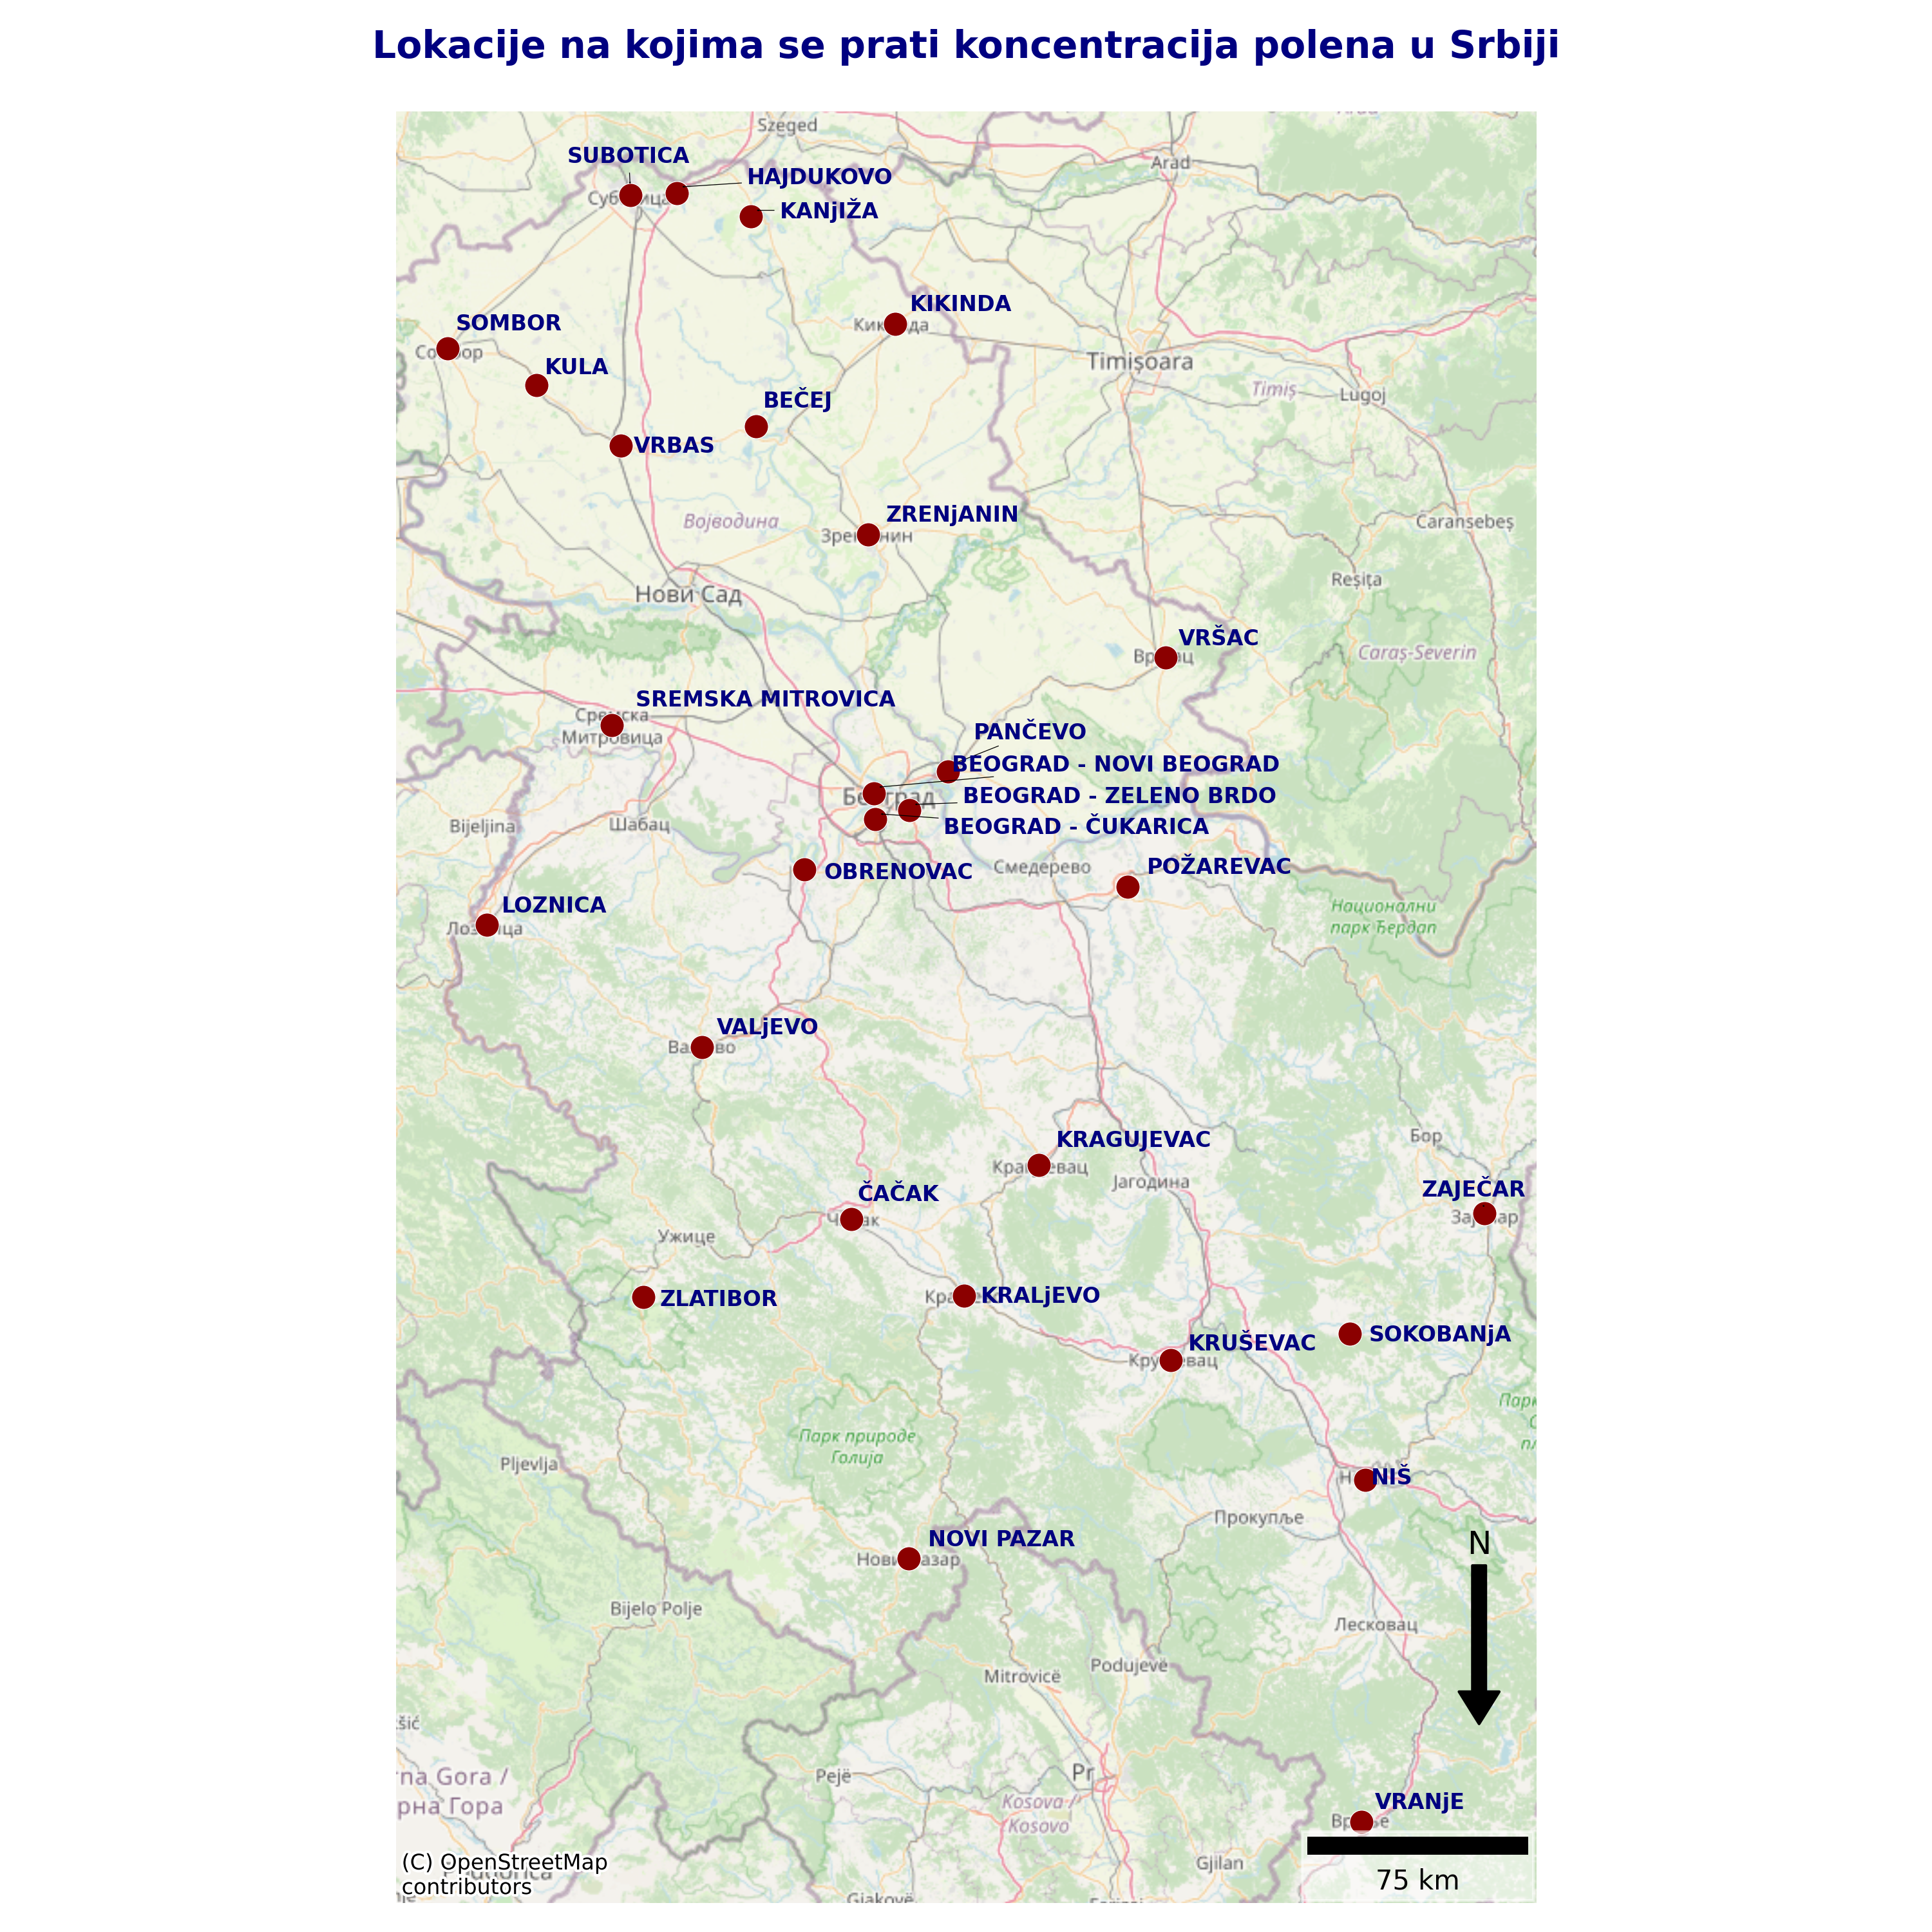
\includegraphics[width=0.6\textwidth]{grafici/mapa_lokacija.png}
    \caption{Lokacije mernih stanica za praćenje koncentracije polena u Srbiji.}
    \label{fig:lokacije_polen_srbija}
\end{figure}

\begin{figure}[H]
    \centering
    % Prvi red
    \subfigure[Ambrozija -- Kragujevac]{%
        \includegraphics[width=0.48\linewidth]{grafici/AMBROZIJA_KRAGUJEVAC_daily_concentration.png}
        %\label{fig:ambrozija_kragujevac}
    }
    \subfigure[Ambrozija -- Pančevo]{%
        \includegraphics[width=0.48\linewidth]{grafici/AMBROZIJA_PANČEVO_daily_concentration.png}
        %\label{fig:ambrozija_pancevo}
    }

    % Drugi red
    \subfigure[Jova -- Kragujevac]{%
        \includegraphics[width=0.48\linewidth]{grafici/JOVA_KRAGUJEVAC_daily_concentration.png}
        %\label{fig:jova_kragujevac}
    }
    \subfigure[Jova -- Pančevo]{%
        \includegraphics[width=0.48\linewidth]{grafici/JOVA_PANČEVO_daily_concentration.png}
        %\label{fig:jova_pancevo}
    }

    % Treći red
    \subfigure[Trave -- Kragujevac]{%
        \includegraphics[width=0.48\linewidth]{grafici/TRAVE_KRAGUJEVAC_daily_concentration.png}
        %\label{fig:trave_kragujevac}
    }
    \subfigure[Trave -- Pančevo]{%
        \includegraphics[width=0.48\linewidth]{grafici/TRAVE_PANČEVO_daily_concentration.png}
        %\label{fig:trave_pancevo}
    }

    \caption{Vremenske serije dnevnih koncentracija polena odabranih alergena u Kragujevcu i Pančevu.}
    \label{fig:subplots_3x2_all}
\end{figure}



\textbf{Meteorološki podaci:}

Meteorološki podaci preuzeti su sa \href{https://cds.climate.copernicus.eu/datasets/reanalysis-era5-single-levels?tab=overview}{Copernicus Climate Data Store}, iz baze ERA5 \textit{"Reanalysis - ERA5 Single Levels"} \cite{hersbach2020}.

Podaci obuhvataju meteorološke varijable sa vremenskom rezolucijom od jednog sata i prostornom rezolucijom od ~31 km, uključujući:

\begin{itemize}
    \item Temperatura vazduha na 2 m (°C)
    \item Relativna vlažnost vazduha (\%)
    \item Brzina vetra (m/s)
    \item Padavine (mm)
    \item Pravac duvanja vetra (rad)
\end{itemize}

Za potrebe analize, podaci su agregirani u dnevne prosečne vrednosti i prostorno interpolirani na lokacije mernih stanica polena.

\subsection{Veza između meteoroloških parametara i koncentracije polena ambrozije}


Analiza zavisnosti između koncentracije polena alergena i meteoroloških parametara sprovedena je za tri lokacije: Kragujevac, Požarevac i Pančevo. Rezultati ukazuju na sledeće obrasce:

\textbf{Temperatura} pokazuje \textbf{slabu pozitivnu korelaciju} sa koncentracijom polena ambrozije na svim lokacijama (r $\approx$ 0.23 – 0.28), dok kod polena jove i trava ova korelacija varira od veoma male do gotovo zanemarljive vrednosti. Konkretno, za travu su vrednosti temperature bile izuzetno niske, dok za jovu na svim lokacijama nisu prelazile r $\approx$ 0.1.

\textbf{Vlažnost vazduha} pokazuje \textbf{slabu negativnu korelaciju} za ambroziju (r $\approx$ -0.2 do -0.23), što je u skladu sa biološkim mehanizmom otežanog širenja polena pri višoj vlažnosti vazduha. Kod jove i trava, korelacije sa vlažnošću su niske i u većini slučajeva statistički neznačajne.

\textbf{Padavine}, \textbf{brzina vetra} i \textbf{pravac vetra} uglavnom pokazuju \textbf{vrlo malu ili zanemarljivu korelaciju} sa koncentracijom polena za sve alergene, sa vrednostima Pirsonovog koeficijenta bliskim nuli.

Ovi rezultati su u skladu sa prethodnim istraživanjima u regionu centralne i jugoistočne Evrope \cite{sofiev2006towards,grewling2016combining,sikoparija2017pannonian}, 
koja ukazuju da temperatura podstiče otpuštanje i emisiju polena, dok viša vlažnost vazduha može otežati širenje polena u vazduhu. Padavine dovode do spiranja polena iz atmosfere, dok brzina i pravac vetra imaju složen nelinearan uticaj, zavisan od pravca transporta i regionalne orografije, koji linearna korelacija ne može u potpunosti da opiše.

S obzirom na to da za padavine, brzinu i pravac vetra \textbf{gotovo da ne postoji linearna veza sa koncentracijom polena}, ovi parametri \textbf{neće biti uzeti u razmatranje prilikom projektovanja linearnih modela}, kao što su \textit{Kriging}, \textit{SARIMAX} i \textit{Prophet}. Međutim, zbog mogućih nelinearnih interakcija, ovi parametri mogu biti \textbf{uključeni u Random Forest modele}, koji su robusniji na ovakve tipove zavisnosti.

\begin{table}[!ht]
    \centering
    \begin{tabular}{|l|l|l|l|l|}
    \hline
        Alergen & Parametar & KRAGUJEVAC & POŽAREVAC & PANČEVO \\ \hline
        \multirow{2}{*}{AMBROZIJA}
        & Temperatura & 0.271 & 0.231 & 0.284 \\ \cline{2-5}
        & Padavine & -0.067 & -0.044 & -0.033 \\ \cline{2-5}
        & Vlažnost vazduha & -0.045 & -0.205 & -0.232 \\ \cline{2-5}
        & Brzina vetra & -0.088 & -0.008 & -0.088 \\ \cline{2-5}
        & Pravac duvanja vetra  & -0.073 & 0.025 & -0.043 \\ \hline
        \multirow{2}{*}{JOVA}
        & Temperatura & 0.097 & 0.054 & 0.023 \\ \cline{2-5}
        & Padavine & -0.062 & -0.084 & -0.053 \\ \cline{2-5}
        & Vlažnost vazduha & -0.138 & -0.072 & -0.058 \\ \cline{2-5}
        & Brzina vetra & 0.071 & 0.026 & 0.015 \\ \cline{2-5}
        & Pravac duvanja vetra  & 0.087 & 0.091 & -0.008 \\ \hline
        \multirow{2}{*}{TRAVE}
        & Temperatura & 0.013 & 0.069 & 0.094 \\ \cline{2-5}
        & Padavine & -0.058 & -0.077 & -0.063 \\ \cline{2-5}
        & Vlažnost vazduha & 0.084 & -0.011 & -0.005 \\ \cline{2-5}
        & Brzina vetra & 0.010 & 0.007 & 0.010 \\ \cline{2-5}
        & Pravac duvanja vetra  & 0.016 & 0.108 & 0.025 \\ \hline
    \end{tabular}
\end{table}




Na slici \ref{fig:ambrozija_meteo_gradovi} prikazana je zavisnost koncentracije polena ambrozije od meteoroloških parametara za sve analizirane lokacije i alergene, zajedno sa regresionim linijama i vrednostima Pirsonovog koeficijenta korelacije za svaku promenljivu.

\begin{figure}[H]
    \centering
    \includegraphics[width=1\textwidth]{grafici/ambrozija_meteo_gradovi.png}
    \caption{Zavisnost koncentracije polena ambrozije od meteoroloških parametara (temperatura, vlažnost vazduha, padavine, brzina i pravac vetra) na analiziranim lokacijama.}
    \label{fig:ambrozija_meteo_gradovi}
\end{figure}


\subsection{Preprocesiranje i čišćenje podataka}

Kako bi analiza bila precizna i pouzdana, podaci o koncentracijama polena najpre su detaljno preprocesirani i očišćeni. Prvi korak u ovom procesu bilo je filtriranje podataka kako bi se u analizi posmatrali samo oni periodi godine koji odgovaraju sezoni cvetanja alergena. Ovakav pristup ima dvostruko opravdanje: s jedne strane, van sezone često nedostaju merenja jer koncentracije polena nisu prisutne u vazduhu, dok s druge strane, upravo je tokom sezone najvažnije imati tačne informacije i predikcije koncentracija zbog uticaja na zdravlje stanovništva \cite{damato2007, who2003}.

Na osnovu informacija sa \href{https://data.gov.rs/sr/datasets/polen-objedinjeni-podatsi-od-2016-godine/}{Portala otvorenih podataka Republike Srbije} sezonski periodi za odabrane alergene su sledeći:

\begin{itemize}
    \item \textbf{Ambrozija}: sezona traje od sredine jula do septembra.
    \item \textbf{Jova}: sezona traje od februara do sredine marta.
    \item \textbf{Trave}: sezona traje od aprila do septembra.
\end{itemize}

Kako bi predikcija bila robusnija i pokrivala potencijalne rane početke i kasne završetke sezona, ovi intervali su u radu blago prošireni i definisani na sledeći način:

\begin{itemize}
    \item \textbf{Ambrozija}: od 9. jul do 1. oktobar
    \item \textbf{Jova}: od 30. januara do 31. mart
    \item \textbf{Trave}: od 30. marta do 1. oktobra
\end{itemize}

Na slici \ref{fig:seasonal_concentration} prikazani su grafikoni koncentracija za odabrane alergene u sezonskim periodima za gradove Kragujevac i Pančevo. 

\begin{figure}[H]
    \centering
    % Prvi red
    \subfigure[Ambrozija – Kragujevac]{%
        \includegraphics[width=0.48\linewidth]{grafici/AMBROZIJA_KRAGUJEVAC_seasonal_concentration.png}
    }
    \subfigure[Ambrozija – Pančevo]{%
        \includegraphics[width=0.48\linewidth]{grafici/AMBROZIJA_PANČEVO_seasonal_concentration.png}
    }

    % Drugi red
    \subfigure[Jova – Kragujevac]{%
        \includegraphics[width=0.48\linewidth]{grafici/JOVA_KRAGUJEVAC_seasonal_concentration.png}
    }
    \subfigure[Jova – Pančevo]{%
        \includegraphics[width=0.48\linewidth]{grafici/JOVA_PANČEVO_seasonal_concentration.png}
    }

    % Treći red
    \subfigure[Trave – Kragujevac]{%
        \includegraphics[width=0.48\linewidth]{grafici/TRAVE_KRAGUJEVAC_seasonal_concentration.png}
    }
    \subfigure[Trave – Pančevo]{%
        \includegraphics[width=0.48\linewidth]{grafici/TRAVE_PANČEVO_seasonal_concentration.png}
    }

    \caption{Sezonske koncentracije polena ambrozije, jove i trava u gradovima Kragujevac i Pančevo.}
    \label{fig:seasonal_concentration}
\end{figure}


\bigskip

\textbf{Transformacija podataka.}

U cilju smanjenja varijanse i stabilizacije disperzije podataka, u analizi će biti primenjene sledeće transformacije:

\begin{itemize}
    \item \textbf{Box-Cox transformacija}: standardna metoda za normalizaciju podataka i smanjenje varijabilnosti varijanse \cite{boxcox1964}.
    \item \textbf{Log transformacija}: transformacija oblika $\log(1 + \frac{x}{30})$, gde je $x$ koncentracija polena. Ova transformacija je izabrana kako bi se najviše rasprostranile vrednosti koncentracija oko 30 zrna/m³, s obzirom na to da ta vrednost predstavlja prag kada kod ljudi dolazi do izraženijih alergijskih simptoma \cite{damato2007}.
    \begin{figure}[H]
        \centering
        \includegraphics[width=0.6\textwidth]{grafici/log1p.png}
        \caption{Primena log transformacije na koncentracije polena ambrozije.}
        \label{fig:log_transform}
    \end{figure}
    
\end{itemize}

Primena ovih transformacija omogućava da modeli predikcije bolje uoče strukturu podataka i umanje uticaj ekstremnih vrednosti, čime se povećava tačnost i stabilnost modela u daljim analizama.

Slika \ref{fig:ambrozija_transforms} prikazuje kako izgleda signal koncentracije polena ambrozije nakon primene različitih transformacija. Na originalnom signalu uočavaju se izraženi pikovi koncentracije tokom sezona cvetanja, sa velikim razlikama između godina. Nakon primene \textit{Box-Cox} transformacije, varijansa signala je značajno smanjena, a raspodela približena normalnoj, što je korisno za primenu linearnih modela. Transformacija $\log(1 + \frac{x}{30})$ posebno ističe vrednosti oko 30 zrna/m³, praga iznad kog koncentracija ambrozije najčešće izaziva alergijske simptome kod osetljivih osoba.
\begin{figure}[H]
    \centering
    \includegraphics[width=1\textwidth]{grafici/AMBROZIJA_POŽAREVAC_seasonal_concentration_transforms.png}
    \caption{Primer uticaja Box-Cox i log transformacije na signal koncentracije polena ambrozije u Požarevcu.}
    \label{fig:ambrozija_transforms}
\end{figure}

\subsection{Imputacija}

U cilju popunjavanja nedostajućih vrednosti koncentracija polena, u ovom radu primenjena je metoda Kriging interpolacije \cite{cressie1993statistics, chiles2009geostatistics}. Proces imputacije sproveden je kroz sledeće korake:

\begin{enumerate}
    \item \textbf{Transformacija podataka.} \\
    Kriging model je primenjen nakon odgovarajućih transformacija podataka kako bi se stabilizovala varijansa i poboljšala prostorno-vremenska interpolacija koncentracija polena. Transformacije su sprovedene na dva različita načina.

    Prvi pristup podrazumevao je direktnu primenu \textit{Box-Cox} ili $\log(1 + \frac{x}{30})$ transformacije na sirove podatke. U ovom slučaju, za \textit{Box-Cox} transformaciju je određivana posebna vrednost parametra $\lambda$ za svaku lokaciju pojedinačno, čime je omogućeno optimalno prilagođavanje distribuciji podataka svake merne stanice.

    \item \textbf{Fitovanje trenda i sezonalnosti.} \\
    Nakon transformacije podataka, sprovedeno je modelovanje determinističkih komponenti koncentracija polena, koje obuhvataju trend i sezonalnost. Trend je modelovan primenom linearne regresije, gde su u model uključeni konstanta  i linearna promena u vremenu, uz mogućnost dodavanja egzogenih promenljivih, poput temperature i vlažnosti vazduha.

    Sezonska komponenta modelovana je pomoću Furijeovih redova opšte forme \cite{hyndman2018forecasting}:

    \[
    S_t = \sum_{k=1}^{K} \alpha_k \sin\left( \frac{2 \pi k t}{T} \right)
    + \beta_k \cos\left( \frac{2 \pi k t}{T} \right),
    \]

    gde je $T$ period sezonalnosti (u ovom slučaju $T=365$, što odgovara godišnjem periodu), $t$ trenutni dan u godini, $\alpha_k$ i $\beta_k$ parametri sinusnih i kosinusnih komponenti, a $K$ broj Furijeovih parova uključenih u model.

    U radu je korišćen broj redova $K=2$, kako bi se izbeglo preobučavanje modela i sačuvala glatkoća sezonske komponente.

    Ovako definisan model omogućava izdvajanje trenda i sezonske strukture iz podataka, čime se preostala komponenta signala (reziduali) može smatrati stacionarnom i pogodnom za dalju analizu. 
    
    \begin{figure}[H]
        \centering
        \includegraphics[width=1\textwidth]{grafici/AMBROZIJA_POŽAREVAC_seasonal_decomposition.png}
        \caption{Sezonska dekompozicija koncentracije polena ambrozije u Požarevcu: trend, sezonalnost i reziduali.}
        \label{fig:seasonal_decomposition}
    \end{figure}

    \item \textbf{Fitovanje variograma.} \\

    Nakon izdvajanja trenda i sezonske komponente, sprovedeno je fitovanje variograma u cilju modelovanja strukture prostorno-vremenske zavisnosti koncentracija polena \cite{cressie1993statistics, chiles2009geostatistics}. U radu je pretpostavljeno da je variogram separabilan, odnosno da se može modelovati kao zbir prostornog i vremenskog variograma.

    Empirijski variogram je izračunavan prema standardnoj formuli:

    \[
    \gamma(h) = \frac{1}{2N(h)} \sum_{i=1}^{N(h)} \left[ z(u_i) - z(u_i + h) \right]^2,
    \]

    gde je $N(h)$ broj parova tačaka razdvojenih rastojanjem $h$, a $z(u_i)$ koncentracija polena u tački $u_i$.

    Za oba variograma (vremenski i prostorni) korišćen je \textbf{eksponencijalni model} \cite{chiles2009geostatistics}, budući da prirodne pojave često najbolje odgovaraju eksponencijalnoj strukturi zavisnosti. Opšta forma eksponencijalnog variograma definisana je izrazom:

    \[
    \gamma(h) = c_0 + c \left( 1 - e^{-\frac{h}{a}} \right),
    \]

    gde je $c_0$ nugget efekt, $c$ sill, $a$ range parametar, a $h$ rastojanje (prostorno ili vremensko).

    \textbf{Vremenski variogram} procenjen je korišćenjem parova posmatranja iz iste lokacije u različitim vremenskim periodima. Diskretizacija je sprovedena sa korakom od \textbf{5 dana}, čime su vremenska kašnjenja grupisana u binove radi stabilnije procene variograma i smanjenja varijabilnosti.

    \textbf{Prostorni variogram} procenjen je korišćenjem parova posmatranja za isti dan na različitim lokacijama. Diskretizacija je u ovom slučaju sprovedena sa korakom od \textbf{40 km}. Budući da su mnoge tačke bile prostorno veoma blizu, grupisane su u iste binove kako bi se izbegla dominacija velikog broja parova sa minimalnim rastojanjima i omogućilo stabilnije fitovanje modela.

    Na osnovu dobijenih prostornog i vremenskog variograma, zajednički (spatio-temporal) variogram određen je prema sledećoj formuli:

    \[
    \gamma(u,v) = \gamma(u,0) + \gamma(0,v) - k \gamma(u,0) \gamma(0,v),
    \]

    gde $\gamma(u,0)$ predstavlja prostorni variogram, $\gamma(0,v)$ vremenski variogram, dok je $k$ parametar koji se određuje optimizacijom kao onaj koji najbolje zadovoljava uslove separabilnosti i pruža najbolji fit spatio-temporal variograma.

     \begin{figure}[H]
        \centering
        \includegraphics[width=1\textwidth]{grafici/AMBROZIJA_variogrami.png}
        \caption{Empirijski i fitovani prostorni i vremenski variogrami koncentracije polena ambrozije.}
        \label{fig:variogrami}
    \end{figure}

    \item \textbf{Interpolacija nedostajućih podataka.} \\

    Nakon fitovanja prostornog i vremenskog variograma, sprovedena je spatial-temoral Kriging interpolacija u cilju procene nedostajućih vrednosti koncentracija polena.

    Da bi se vremenska komponenta mogla upoređivati i kombinovati sa prostornim rastojanjima u prostorno-vremenskom modelovanju, izvršeno je skaliranje vremenskih razlika faktorom $a_s / a_t$, gde je $a_s$ prostorni range, a $a_t$ vremenski range parametar variograma. Vrednosti ovog faktora su \textbf{ograničene na interval 10–50}, kako bi se izbegle ekstremne vrednosti i obezbedilo da u modelu \textbf{jedan dan odgovara prostornom rastojanju između približno 10 i 50 km}. Ovakvo ograničenje je uvedeno kako bi se sprečile nerealistično velike ili male vrednosti skaliranja, koje bi narušile balans između prostorne i vremenske komponente u modelu. Konkretno, prevelike vrednosti bi dovele do toga da se promene u vremenu posmatraju kao zanemarljive u poređenju sa prostorom, dok bi premale vrednosti učinile da vremenska komponenta potpuno nadjača prostornu strukturu podataka.

    Za procenu reziduala koncentracije u nekoj tački, korišćene su \textbf{najbliže poznate vrednosti} po prostorno-vremenskoj distanci, pri čemu je maksimalno rastojanje za uključivanje u predikciju bilo ograničeno na \textbf{200 km}. Ukoliko za neku tačku nije bilo dovoljno poznatih posmatranja koja ispunjavaju ovaj uslov, pretpostavljano je da je rezidual jednak nuli, te je \textbf{konačna procena koncentracije} za tu tačku dobijena kao zbir prethodno fitovanog trenda i sezonske komponente.

    Na kraju ovog dela, primenjeno je \textbf{winsorizing} (ograničavanje ekstremnih vrednosti) reziduala \cite{jones1996winsorizing}, kako bi se smanjio uticaj izuzetno visokih vrednosti koje bi mogle narušiti stabilnost modela i dovesti do nerealnih predikcija koncentracije polena.
    
    Konkretno, za svaku lokaciju izračunati su prvi ($Q1$) i treći kvartil ($Q3$) reziduala, kao i interkvartilni raspon ($IQR = Q3 - Q1$). Na osnovu toga je određena gornja granica, definisana kao $Q3 + IQR$. Sve vrednosti reziduala koje su prelazile ovu granicu zamenjene su upravo tom graničnom vrednošću.

    \item \textbf{Rekonstrukcija konačnih vrednosti.} \\

    Poslednji korak u procesu imputacije je dobijanje konačnih procena koncentracija polena. To je postignuto jednostavnim sabiranjem prethodno procenjenih komponenti – trenda i sezonalnosti, zajedno sa imputiranim rezidualima dobijenim Kriging interpolacijom \cite{cressie1993statistics}.

    Nakon toga, na dobijene vrednosti primenjena je \textbf{inverzna transformacija}, odnosno obrnuti postupak transformacija opisanih u prvom koraku (\textit{Box-Cox} ili $\log(1 + \frac{x}{30})$ transformacija), kako bi se rezultati vratili u originalnu skalu koncentracija polena (zrna/m³).

    \item \textbf{Evaluacija modela.} \\

    Nakon rekonstrukcije konačnih vrednosti, sprovedena je evaluacija performansi Kriging modela kako bi se procenila njegova tačnost i generalizacija. 

    U radu je primenjena \textbf{5-fold cross-validation} metoda \cite{hyndman2018forecasting}. Za svaki alergen, kompletan skup podataka podeljen je na pet podskupova (foldova). U svakoj iteraciji, model je treniran na četiri podskupa, dok je preostali podskup korišćen za evaluaciju. Ovaj postupak ponovljen je pet puta, tako da je svaki podskup jednom korišćen kao test skup. 

\end{enumerate}

\subsection{Modelovanje vremenske serije i podešavanje parametara SARIMAX modela}

Za modelovanje i predikciju koncentracija polena korišćen je SARIMAX model, koji omogućava istovremeno opisivanje sezonskih obrazaca u podacima i uključivanje dodatnih meteoroloških faktora kao prediktora, poput temperature i vlažnosti vazduha \cite{box1970, brockwell2002, hyndman2018forecasting}.

Modelovanje je sprovedeno kroz sledeće korake:

\begin{enumerate}
    \item \textbf{Priprema podataka.} \\
    Kao ulaz u SARIMAX model korišćeni su prethodno imputirani podaci, na koje je primenjena jedna od transformacija opisanih u ranijim koracima (\textit{Box-Cox} ili $\log(1 + \frac{x}{30})$ transformacija). Ove transformacije su korišćene u cilju smanjenja varijanse i postizanja stacionarnosti podataka, što je preduslov za stabilno i precizno modelovanje vremenskih serija.

    Serija je vizuelno analizirana radi procene potrebe za diferencijacijom. S obzirom na to da su koncentracije polena posmatrane u periodu od deset godina, tokom kojeg se ne očekuje postojanje značajnog linearnog ili sezonskog trenda, odlučeno je da se parametri diferenciranja fiksiraju na $d=0$ i $D=0$.
    Pored vizuelne analize, stacionarnost serije je dodatno testirana uz pomoć statističkih testova \textit{ADF} i \textit{KPSS}, koji su opisani u odeljku~\ref{sec:stationarity}.


    \item \textbf{Određivanje perioda sezonalnosti.} \\
    Budući da su iz analize izostavljeni periodi van sezona cvetanja, standardna godišnja sezonalnost (npr. 365 dana) nije mogla biti direktno korišćena u modelu. Jedno od potencijalnih rešenja bilo bi da se za datume van sezone unesu vrednosti nula, čime bi model formalno mogao da koristi godišnji period. Međutim, time bi SARIMAX model bio pristrasan ka predviđanju nižih koncentracija, smanjila bi se preciznost procene sezonskih amplituda, a kvalitet predikcija u sezonskim periodima bio bi značajno degradiran.

    \begin{figure}[H]
        \centering
        \includegraphics[width=0.6\textwidth]{grafici/periodogram_AMBROZIJA_POŽAREVAC.png}
        \caption{Periodogram koncentracija polena ambrozije u Požarevcu, korišćen za određivanje dominantnog sezonskog perioda.}
        \label{fig:periodogram_ambrozija}
    \end{figure}
    Zbog toga je za određivanje sezonskog perioda korišćen \textbf{maksimalni pik periodograma} vremenske serije \cite{yule1927, slutsky1937}. Ovim pristupom, dominantna frekvencija u podacima određena je na osnovu realnih obrazaca, a ne unapred nametnutih sezonskih pretpostavki, što omogućava modelu da preciznije uhvati specifične sezonske fluktuacije koncentracija polena.


    \item \textbf{Definisanje strukture modela.} \\
    SARIMAX model karakterišu nesezonski parametri (p, d, q), sezonski parametri (P, D, Q, s), kao i egzogene promenljive \cite{box1970, brockwell2002}. U ovom radu, vrednosti d i D su fiksirane na 0, dok su ostali parametri određivani kombinacijom sledećih metoda:
    \begin{itemize}
        \item Vizuelne analize ACF i PACF grafova za inicijalnu procenu potencijalnih vrednosti p, q, P i Q.
        \item Grid search procedure, uz minimizaciju AICc kriterijuma, radi pronalaženja optimalne kombinacije parametara i izbegavanja preobučavanja modela \cite{burnham2002}.
    \end{itemize}

    Kao egzogene promenljive u model su uključivani \textbf{Furijeovi redovi reda 3}, kako bi se modelovala sezonalnost bez rizika od preobučavanja, kao i potencijalno meteorološki podaci (temperatura, vlažnost vazduha) za poboljšanje prediktivne sposobnosti modela.

    
    \begin{figure}[H]
        \centering
        \includegraphics[width=1\textwidth]{grafici/seasonal_segment_AMBROZIJA_POŽAREVAC.png}
        \caption{STL dekompozicija vremenske serije koncentracije polena ambrozije: prikaz originalnih podataka, izdvojenog trenda, sezonske komponente i reziduala, uz ACF i PACF signala korišćenih za inicijalnu procenu parametara SARIMAX modela.}
        \label{fig:seasonal_segment_ambrozija}
    \end{figure}

    \item \textbf{Trening modela i rolling forecast evaluacija.} \\
    Model je treniran na podacima iz perioda do kraja 2023. godine. Na osnovu ovih podataka određeni su optimalni modela (p, q, P i Q), uz primenu kriterijuma minimizacije AICc.

    Evaluacija modela sprovedena je za 2024. godinu korišćenjem \textbf{rolling forecast} pristupa \cite{bergmeir2012use}. Ovaj pristup podrazumeva da se, nakon svakog novog posmatranja u tekućoj godini, model refituje i koristi za predikciju koncentracija polena za narednih nekoliko dana unapred. Na taj način simuliran je realni operativni scenario, gde se modeli svakodnevno ažuriraju najnovijim merenjima i koriste za kratkoročne prognoze u cilju pravovremenog informisanja javnosti i zdravstvenih sistema.

    \item \textbf{Rekonstrukcija predikcija.} \\
    Konačne predikcije dobijene su primenom inverzne transformacije (\textit{Box-Cox} ili $\log(1 + \frac{x}{30})^{-1}$, u zavisnosti od prethodno korišćene transformacije) na prediktovane vrednosti modela, čime su rezultati vraćeni u originalnu skalu koncentracija polena (zrna/m³).

    \item \textbf{Metrike evaluacije.} \\
    Evaluacija tačnosti SARIMAX modela sprovedena je korišćenjem metrika definisanih u posebnom odeljku \ref{sec:evaluation_metrics}.

\end{enumerate}

\subsection{Modelovanje vremenske serije korišćenjem Prophet modela}

U cilju predikcije koncentracija polena, pored SARIMAX modela, primenjen je i \textbf{Prophet} model \cite{taylor2018}, razvijen od strane Facebook Research tima.

Proces modelovanja Prophet-om sastojao se od sledećih koraka:

\begin{enumerate}
    \item \textbf{Transformacija podataka.} \\
    Za razliku od nekih drugih modela vremenskih serija, Prophet može efikasno raditi i bez prethodnih transformacija podataka. U ovom radu, model je treniran na podacima unutar sezonskih perioda, koristeći prethodno imputirane vrednosti koncentracija polena. Takođe, kao i u prethodnim analizama, primenjivane su i transformacije (\textit{Box-Cox} ili $\log(1 + \frac{x}{30})$), kako bi se ispitalo da li transformacije dodatno poboljšavaju performanse modela.

    \item \textbf{Definisanje strukture modela.} \\
    Struktura Prophet modela podešavana je optimizacijom sledećih hiperparametara:
    \begin{itemize}
        \item \textbf{changepoint\_prior\_scale}: [0.1, 0.2, 0.5] – kontroliše fleksibilnost modela u detektovanju promena trenda. Niže vrednosti daju glatkiji trend, dok veće omogućavaju praćenje naglih promena u seriji, što je važno za alergene sa izraženim varijacijama.
        \item \textbf{seasonality\_prior\_scale}: [1.0, 2.0, 5.0] – određuje koliko sezonalnost utiče na predikciju. Veće vrednosti omogućavaju veću slobodu sezonskim komponentama, poboljšavajući fit kod alergena sa izraženim sezonskim šablonima.
        \item \textbf{seasonality\_mode}: ['additive', 'multiplicative'] – definiše da li je sezonalnost aditivna (konstantna amplituda) ili multiplikativna (amplituda proporcionalna nivou serije).
        \item \textbf{changepoint\_range}: [0.6, 0.8, 0.95] – definiše proporciju podataka unutar koje model detektuje tačke promene trenda. Veće vrednosti omogućavaju detekciju promena i u kasnijim delovima serije, što je korisno za alergene sa dugom sezonom cvetanja.
    \end{itemize}

    U model je dodat i \textbf{godišnji sezonski efekat}, aproksimiran korišćenjem Furijeovih redova \cite{hyndman2018forecasting}, što omogućava preciznije hvatanje sezonskih obrazaca koncentracije polena tokom godine. Takođe, kao egzogene promenljive uključeni su i meteorološki podaci (npr. temperatura i vlažnost vazduha), kako bi se unapredila prediktivna sposobnost modela.

    Optimalni hiperparametri birani su korišćenjem grid search procedure na podacima do kraja 2023. godine, dok je evaluacija modela sprovedena na podacima iz 2024. godine.



    \item \textbf{Treniranje modela i rolling forecast evaluacija.} \\
    Model je treniran i evaluiran primenom \textbf{rolling forecast} pristupa, kojim se simulira realni operativni scenario predikcije \cite{bergmeir2012use}. Nakon svakog novog posmatranja u tekućoj godini (2024), model je refitovan i korišćen za predikciju koncentracija polena za narednih nekoliko dana unapred.

    Trening je sproveden na dva načina:
    \begin{itemize}
        \item Prvi pristup uključivao je korišćenje svih dostupnih poznatih vrednosti u trening skupu, kako bi model naučio dugoročne obrasce i sezonske fluktuacije koncentracija polena.
        \item Drugi pristup ograničavao je trening skup samo na posmatranja unutar \textbf{±30 dana} oko datuma predikcije svake godine. Ovakav pristup omogućava modelu da se fokusira na lokalne sezonske obrasce specifične za posmatrani period godine, s obzirom na to da koncentracije polena u različitim mesecima imaju različite obrasce i amplitudu.
    \end{itemize}

    \item \textbf{Metrike evaluacije.} \\
    Metrike korišćene za evaluaciju performansi Prophet modela detaljno su opisane u odeljku \ref{sec:evaluation_metrics}, gde su predstavljeni RMSLE, MAE, RMSE, kao i dodatne evaluacije na osnovu klasifikacije koncentracija i predikcije datuma početka sezone.

\end{enumerate}

\subsection{Modelovanje koncentracija polena korišćenjem Random Forest modela}

Za predikciju koncentracija polena primenjen je i Random Forest (RF) model \cite{breiman2001}.
Sam proces modelovanja se sastoji iz sledećih koraka:

\begin{enumerate}
    \item \textbf{Transformacija podataka.} \\
    Za razliku od linearnih modela vremenskih serija, Random Forest može efikasno raditi i bez prethodnih transformacija podataka. U ovom radu, model je treniran na podacima unutar sezonskih perioda, koristeći prethodno imputirane vrednosti koncentracija polena. Takođe, kao i u prethodnim analizama, primenjivane su i transformacije (\textit{Box-Cox} ili $\log(1 + \frac{x}{30})$), kako bi se ispitalo da li transformacije dodatno poboljšavaju performanse modela \cite{boxcox1964}.

    \item \textbf{Uključivanje dodatnih promenljivih.} \\
    Budući da Random Forest ne pretpostavlja linearnost odnosa između prediktora i ciljne promenljive, u model su uključene i druge meteorološke promenljive, kao što su brzina vetra, pravac vetra, padavine, temperatura i vlažnost vazduha, kako bi se obuhvatile sve potencijalno relevantne informacije za predikciju koncentracija polena.

    \item \textbf{Podešavanje hiperparametara modela.} \\
    Optimalni parametri modela određivani su korišćenjem grid search procedure, pri čemu su testirane sledeće vrednosti:
    \begin{itemize}
        \item \textbf{n\_estimators}: [250] – broj stabala u šumi; veći broj smanjuje varijansu modela, ali povećava vreme treniranja.
        \item \textbf{max\_depth}: [5, 10, None] – maksimalna dubina svakog stabla; manja dubina smanjuje mogućnost preobučavanja.
        \item \textbf{max\_features}: ['log2', 'sqrt'] – broj prediktora razmatranih pri svakom split-u; koristi se log2 ili kvadratni koren broja prediktora radi smanjenja korelacije među stablima.
        \item \textbf{min\_samples\_split}: [2, 5] – minimalni broj uzoraka potreban za podelu čvora; veće vrednosti smanjuju kompleksnost stabla.
        \item \textbf{max\_lag}: [3, 5] – maksimalni broj vremenskih lagova uključenih kao prediktora u model.
    \end{itemize}

    \item \textbf{Feature engineering.} \\
    Kao ulazni prediktori u model su uključeni:
    \begin{itemize}
        \item vrednosti koncentracije polena sa zaostatkom do $max\_lag$ dana (lag features),
        \item prosečna koncentracija u prethodnih 7 dana,
        \item prosečna koncentracija u istom periodu prethodne godine ($\pm$ 3 dana),
        \item koncentracija na isti dan prethodne godine,
        \item broj dana od početka sezone te godine i godina,
        \item Furijeovim redovi reda 2, sa periodom određivanim na isti način kao kod SARIMAX modela, radi aproksimacije sezonskih obrazaca \cite{yule1927, slutsky1937}.
    \end{itemize}

    \item \textbf{Treniranje i evaluacija modela.} \\
    Optimalni parametri modela birani su na podacima do kraja 2023. godine, dok je evaluacija sprovedena na podacima iz 2024. godine, korišćenjem \textbf{rolling forecast} pristupa \cite{bergmeir2012use}. Ovaj pristup podrazumeva da se nakon svakog novog posmatranja u tekućoj godini model ažurira i koristi za predikciju koncentracija polena za narednih nekoliko dana unapred, čime se simulira realni operativni scenario.

    Budući da pri rolling forecast predikciji nisu uvek dostupne sve vrednosti za lag prediktore (npr. prilikom predikcije za dva dana unapred nije poznata vrednost koncentracije za dan+1), ovaj problem je rešen korišćenjem prethodno predikovanih vrednosti modela kao ulaza za naredne korake predikcije.

    \item \textbf{Metrike evaluacije.} \\
    Metrike korišćene za evaluaciju performansi Random Forest modela detaljno su opisane u odeljku \ref{sec:evaluation_metrics}, gde su predstavljeni RMSLE, MAE, RMSE, kao i dodatne evaluacije na osnovu klasifikacije koncentracija i predikcije datuma početka sezone.
\end{enumerate}

\subsection{Metrike evaluacije modela}
\label{sec:evaluation_metrics}

Za proveru ispravnosti modela, pre same evaluacije performansi, ispitivano je da li reziduali predstavljaju beli šum primenom \textit{Ljung–Box testa} \cite{ljung1978}. Rezultati su pokazali da su reziduali nekorelisani kod svih primenjenih modela, što potvrđuje njihovu konzistentnost, iako ova analiza nije dalje detaljno razmatrana u okviru ovog rada.

Za evaluaciju performansi modela vremenskih serija korišćene su standardne metrike koje omogućavaju procenu odstupanja predikcija od stvarnih vrednosti, kao i dodatne metrike vezane za sezonalnost i klasifikaciju koncentracija polena. U ovom radu fokus je stavljen na sledeće metrike:

\begin{itemize}
    \item \textbf{Root Mean Squared Logarithmic Error (RMSLE)} \\
    RMSLE naglašava proporcionalne greške i posebno je pogodan za podatke sa velikim varijacijama i ekstremnim vrednostima, kakvi su podaci o koncentraciji polena. Definiše se kao:
    \[
    RMSLE = \sqrt{ \frac{1}{n} \sum_{i=1}^{n} ( \log(1 + \frac{\hat{y}_i}{30}) - \log(1 + \frac{y_i}{30}) )^2 },
    \]
    gde su $\hat{y}_i$ prediktovane vrednosti, a $y_i$ posmatrane vrednosti koncentracije polena. Ova metrika omogućava da se greške pri malim vrednostima tretiraju proporcionalno značajno, dok se uticaj velikih ekstremnih odstupanja ublažava \cite{brockwell2002,hyndman2018forecasting}.

    \item \textbf{Mean Absolute Error (MAE)} \\
    MAE predstavlja prosečno apsolutno odstupanje predikcija od stvarnih vrednosti i često se koristi zbog svoje intuitivnosti i robusnosti prema ekstremnim vrednostima.

    \item \textbf{Root Mean Squared Error (RMSE)} \\
    RMSE kvadrira odstupanja, pa veću težinu daje većim greškama. Koristi se kao dopuna MAE kako bi se ocenilo koliko su predikcije podložne velikim odstupanjima.
    
    \item \textbf{Klasifikacija koncentracija} \\
    Pored standardnih regresionih metrika, izvršena je i klasifikacija koncentracija polena. Definisane su tri kategorije:
    \begin{itemize}
        \item \textbf{Niska} — vrednosti manje od donje granične vrednosti.
        \item \textbf{Srednja} — vrednosti između donje i gornje granične vrednosti.
        \item \textbf{Visoka} — vrednosti veće od gornje granične vrednosti.
    \end{itemize}
    Ova klasifikacija omogućava praktičnu evaluaciju modela u smislu korisnosti za zdravstveni sistem i javnost, jer kategorizovane vrednosti imaju direktan uticaj na zdravstvene preporuke.

    \item \textbf{Predikcija datuma početka sezone} \\
    Posebna metrika odnosila se na tačnost predikcije datuma početka sezone polena. 
    \begin{itemize}
        \item \textbf{Stvarna vrednost} početka sezone definisana je kao prvi dan kada vremenska serija pokazuje koncentraciju veću od donje granice u \emph{tri uzastopna dana}.
        \item \textbf{Predikcija} je vršena tako što je svakog dana model radio prognozu za 7., 8. i 9. dan unapred. Prvi trenutak kada su sve tri prognozirane vrednosti bile iznad donje granice smatran je početkom sezone, pri čemu je kao zvanični datum uzet sedmi dan iz tog intervala.
    \end{itemize}
    Ova metrika omogućava kvantifikaciju sposobnosti modela da pravovremeno identifikuje početak sezone, što je od posebne važnosti za preventivne mere.
\end{itemize}



\newpage
\section{Rezultati}

\subsection{Imputacija}

Za sve alergene sprovedena je detaljna evaluacija različitih metoda za imputaciju nedostajućih vrednosti koncentracija polena, međutim, u ovom radu biće prikazani rezultati samo za tri alergena: ambroziju, jovu i trave. Kao metrika greške korišćen je \textbf{RMSLE (Root Mean Squared Logarithmic Error)}.

\subsubsection{Metodologija evaluacije}

Za evaluaciju imputacionih modela korišćena je \textbf{5-fold cross-validation} procedura \cite{bergmeir2012use}. 
Svi dostupni podaci su podeljeni na pet podskupova (foldova). Trening modela vršen je na četiri folda, dok je performansa evaluirana na preostalom foldu. 
Ovaj proces je ponovljen pet puta, tako da je svaki fold korišćen kao test set jednom, a rezultati su agregirani za svaki alergen posebno.

\vspace{0.3cm}
\noindent \paragraph{\textbf{Upoređene metode imputacije:}}

\begin{itemize}
    \item \textbf{SpatioTemporal Kriging (ST Kriging)} – klasičan spatial-temporal Kriging \cite{cressie1993statistics, chiles2012geostatistics} nakon transformacije podataka \textit{Box-Cox} ili $log(1+\tfrac{x}{30})$.
    \item \textbf{Standardizovani ST Kriging} – podaci standardizovani po lokaciji i alergenu, zatim transformisani (\textit{Box-Cox} ili $log(1+\tfrac{x}{30})$).
    \item \textbf{Standardizovani ST Kriging sa egzogenim promenljivama} – dodat je uticaj temperature i vlažnosti vazduha.
    \item \textbf{Naive Temporal Nearest} – imputacija nedostajuće vrednosti korišćenjem najbliže poznate vremenske vrednosti.
    \item \textbf{IDW (Inverse Distance Weighting)} – metoda imputacije koja koristi prostornu interpolaciju inverznim ponderisanjem po udaljenosti unutar istog dana \cite{shepard1968two}, a u slučaju nedostatka suseda koristi vrednost sa najbližeg datuma iste lokacije.
\end{itemize}


\subsubsection{Rezultati po alergenima}

\paragraph{Ambrozija.}
Za ambroziju, najniži RMSLE postignut je standardizovanim ST Kriging modelom sa \textit{Box-Cox} transformacijom, iznoseći \textbf{0.260 ($\sigma$ = 0.011)}. Slične rezultate dali su i standardizovani modeli sa \textit{Box-Cox}  transformacijom i dodatim egzogenim promenljivama. Naivna metoda imala je RMSLE od 0.309 ($\sigma$ = 0.007), dok je IDW metoda imala značajno višu grešku od 1.085 ($\sigma$ = 0.009).

\paragraph{Jova.}
Za jovu, najbolji rezultat postignut je standardizovanim ST Kriging modelom sa \textit{Box-Cox} transformacijom, sa RMSLE od \textbf{0.244 ($\sigma$ = 0.017)}. Najlošiji rezultat imao je IDW metod sa RMSLE od 0.567 ($\sigma$ = 0.024), dok je naivna metoda dala RMSLE od 0.349 ($\sigma$ = 0.020).

\paragraph{Trave.}
Kod trava, najniži RMSLE postignut je standardizovanim ST Kriging modelom sa \textit{Box-Cox} transformacijom, iznoseći \textbf{0.201 ($\sigma$ = 0.008)}. Naivna metoda dala je RMSLE od 0.231 ($\sigma$ = 0.004), dok je IDW metoda pokazala značajno lošiju tačnost sa RMSLE od 0.437 ($\sigma$ = 0.004).



\begin{table}[H]
\centering
\caption{Rezultati imputacije nedostajućih vrednosti koncentracije polena (RMSLE sa standardnom devijacijom) za različite metode i alergene.}

\label{tab:imputation_all_methods_std}
\renewcommand{\arraystretch}{1.3}
\begin{tabular}{|l|c|c|c|}
\hline
\textbf{Metoda} & \textbf{Ambrozija} & \textbf{Jova} & \textbf{Trave} \\
\hline
ST Kriging (Box-Cox) & 0.336 (0.125) & 0.290 (0.081) & 0.238 (0.063) \\
\hline
ST Kriging (log) & 0.373 (0.155) & 0.289 (0.017) & 0.206 (0.002) \\
\hline
Standardizovani ST Kriging (Box-Cox) & 0.260 (0.011) & 0.244 (0.017) & 0.201 (0.008) \\
\hline
Standardizovani ST Kriging (log) & 0.307 (0.010) & 0.300 (0.013) & 0.223 (0.002) \\
\hline
Standardizovani ST Kriging + exog (Box-Cox) & 0.262 (0.011) & 0.244 (0.017) & 0.201 (0.008) \\
\hline
Standardizovani ST Kriging + exog (log) & 0.322 (0.013) & 0.302 (0.013) & 0.225 (0.003) \\
\hline
Naive Temporal Nearest & 0.309 (0.007) & 0.349 (0.020) & 0.231 (0.004) \\
\hline
IDW Temporal Fallback & 1.085 (0.009) & 0.567 (0.024) & 0.437 (0.004) \\
\hline
\end{tabular}
\end{table}

\begin{figure}[H]
    \centering
    \subfigure{\includegraphics[width=0.48\linewidth]{grafici/AMBROZIJA_KRAGUJEVAC_imputed_concentration.png}}
    \subfigure{\includegraphics[width=0.48\linewidth]{grafici/AMBROZIJA_PANČEVO_imputed_concentration.png}}
    \subfigure{\includegraphics[width=0.48\linewidth]{grafici/JOVA_KRAGUJEVAC_imputed_concentration.png}}
    \subfigure{\includegraphics[width=0.48\linewidth]{grafici/JOVA_PANČEVO_imputed_concentration.png}}
    \subfigure{\includegraphics[width=0.48\linewidth]{grafici/TRAVE_KRAGUJEVAC_imputed_concentration.png}}
    \subfigure{\includegraphics[width=0.48\linewidth]{grafici/TRAVE_PANČEVO_imputed_concentration.png}}
    \caption{Vizuelni prikaz imputacije koncentracija polena za ambroziju, jovu i trave na odabranim lokacijama.}
    \label{fig:imputacija}

\end{figure}



\subsubsection{Diskusija}

Na osnovu dobijenih rezultata, može se zaključiti da je \textbf{standardizovani spatio-temporal Kriging model sa Box-Cox transformacijom} pokazao najniže RMSLE vrednosti za sve analizirane alergene, što ukazuje na njegovu superiornost u imputaciji nedostajućih podataka o koncentraciji polena. Ovaj pristup omogućava stabilizaciju varijanse i bolje prilagođavanje raspodeli podataka, dok standardizacija dodatno uklanja uticaj različitih opsega koncentracija između lokacija.

Analizom uticaja egzogenih promenljivih, konkretno temperature i vlažnosti vazduha, uočeno je da modeli sa i bez ovih kovarijata daju gotovo identične rezultate. S obzirom na to, za praktičnu implementaciju preporučuje se korišćenje modela bez egzogenih promenljivih zbog jednostavnije primene i manjih zahteva za eksternim podacima. Ovakav rezultat može se objasniti činjenicom da su prostorne i vremenske zavisnosti koncentracija polena, koje Kriging model uspešno hvata, delimično već povezane sa meteorološkim faktorima, zbog čega eksplicitno uključivanje temperature i vlažnosti vazduha ne doprinosi značajnom poboljšanju tačnosti predikcija.

Sa druge strane, metoda \textbf{IDW Temporal Fallback} pokazala je značajno slabije performanse u poređenju sa ostalim modelima. Razlog za to leži u njenom konceptualnom ograničenju, jer se oslanja isključivo na prostornu interpolaciju inverznim ponderisanjem po udaljenosti unutar istog dana, a u slučaju nedostatka prostorno bliskih merenja pribegava fallback strategiji uzimanja vrednosti sa najbližeg datuma iste lokacije. Ovakav pristup ne uspeva da adekvatno modeluje složene prostorno-vremenske obrasce distribucije polena, što dovodi do znatno većih grešaka.

Važno je istaći i specifičnost načina prikupljanja podataka – merenja su vršena kontinuirano, sa uzastopnim dnevnim uzorkovanjima koncentracije polena. Zbog toga postoji izražena vremenska autokorelacija između dva uzastopna dana, što objašnjava relativno dobre rezultate \textbf{naivne metode}, koja imputaciju zasniva na najbližem vremenskom susedu. Ipak, rezultati pokazuju da \textbf{spatio-temporal Kriging} uspeva da nadmaši i ovu metodu, zahvaljujući sposobnosti da istovremeno uvaži i prostornu i vremensku zavisnost u predikciji koncentracija polena.

\subsection{Predikcija}

U ovom poglavlju predstavljeni su rezultati predikcije koncentracije polena korišćenjem tri različita modela: \textbf{SARIMAX} \cite{box1970, hyndman2018forecasting}, \textbf{Prophet} \cite{taylor2018}, i \textbf{Random Forest} \cite{breiman2001}, uz poređenje sa \textbf{naivnom metodom} kao baznom linijom. Rezultati poređenja prikazani su u tabelama \ref{tab:rlmsle_ambrozija} i \ref{tab:rlmsle_jova}.

\subsubsection{Metodologija evaluacije}

Za evaluaciju je korišćen \textbf{rolling forecast} pristup \cite{bergmeir2012use}, kojim se simulira realni scenario operativnog predviđanja, gde su podaci dostupni samo do trenutka predikcije. Modeli su trenirani na podacima do kraja 2023. godine, dok je evaluacija sprovedena na podacima iz 2024. godine. 

Kao transformacije podataka razmatrane su \textbf{Box-Cox} \cite{boxcox1964}, \textbf{$log(1 + \frac{x}{30})$} i scenario bez transformacije.\footnote{Kod SARIMAX modela transformacija je obavezna.}  
Predikcije su pravljene sa i bez korišćenja meteoroloških promenljivih, kako bi se procenio njihov uticaj na performanse modela.  

Evaluacija performansi modela sprovedena je korišćenjem metrika definisanih u odeljku \ref{sec:evaluation_metrics} \cite{brockwell2002, hyndman2018forecasting}.

\subsubsection{SARIMAX}


\paragraph{\textbf{Optimalni parametri.}}  
Tabela \ref{tab:sarimax_params} prikazuje optimalne SARIMAX parametre za Kragujevac, za ambroziju, za obe transformacije (log i \textit{Box-Cox}) i za modele sa i bez meteoroloških podataka.  
Važno je napomenuti da \textbf{AICc kriterijum nije direktno uporediv između različitih transformacija}, tako da se obe transformacije posebno testiraju, pa se naknadno razmatra  prikladniji model.  

\renewcommand{\arraystretch}{1.3}

\begin{table}[h!]
    \label{tab:sarimax_params}
\centering
\caption{Optimalni SARIMAX parametri za Požarevac (ambrozija) sa različitim transformacijama, meteorološkim parametrima i Furijeovim redom.}


\begin{tabular}{|l|c|c|c|c|c|c|c|c|c|c|c|c|}
\hline
\textbf{Transformacija} & \textbf{Meteo} & $p$ & $d$ & $q$ & $P$ & $D$ & $Q$ & $s$ & \textbf{Fourier($k$)} & AICc & \textbf{T} & \textbf{H} \\ \hline
log    & Da & 2 & 0 & 1 & 1 & 0 & 1 & 85 & 3 & 361.56 & 0.000 & 0.371  \\ \hline
log    & Ne & 2 & 0 & 2 & 1 & 0 & 0 & 85 & 3 & 388.70 & -- & -- \\ \hline
Box-Cox & Da & 2 & 0 & 1 & 1 & 0 & 1 & 85 & 3 & 1801.26 & 0.767 & 0.000 \\ \hline
Box-Cox & Ne & 2 & 0 & 2 & 1 & 0 & 1 & 85 & 3 & 1805.45 & -- & -- \\ \hline
\end{tabular}

\vspace{0.2cm}
\footnotesize{T = temperatura, H = vlažnost vazduha. P-vrednosti označavaju statističku značajnost meteoroloških kovarijata u modelu.}
\end{table}

\paragraph{\textbf{Performanse modela po transformaciji.}}  
Za detaljniju analizu, RMSLE vrednosti su prikazane posebno za Log i \textit{Box-Cox} transformaciju, uz razdvajanje po gradovima, vrstama polena (ambrozija i jova) i po tome da li su meteorološki parametri uključeni u model ili ne.  
Tabela \ref{tab:rmsle_log} prikazuje rezultate za Log transformaciju, dok tabela \ref{tab:rmsle_boxcox} sadrži RMSLE vrednosti za \textit{Box-Cox} transformaciju.  
Na ovaj način može se jasno uočiti kako izbor transformacije i prisustvo meteoroloških kovarijata utiče na preciznost predikcije, kao i razlike u grešci između predikcije za 1 i 7 dana unapred.

%--------------------- Tabela za Log transformaciju ---------------------%
\begin{table}[h!]
\centering
\caption{RMSLE vrednosti za Log transformaciju (1 i 7 dana unapred, sa i bez meteo)}
\begin{tabular}{|l|c|c|c|c||c|c|c|c|}
\hline
\label{tab:rmsle_log}
\multirow{3}{*}{\textbf{Grad}} 
& \multicolumn{4}{c||}{\textbf{Ambrozija}} 
& \multicolumn{4}{c|}{\textbf{Jova}} \\ \cline{2-9}
& \multicolumn{2}{c|}{\textbf{Sa meteo}} & \multicolumn{2}{c||}{\textbf{Bez meteo}} 
& \multicolumn{2}{c|}{\textbf{Sa meteo}} & \multicolumn{2}{c|}{\textbf{Bez meteo}} \\ \cline{2-9}
& \textbf{1 dan} & \textbf{7 dana} & \textbf{1 dan} & \textbf{7 dana} 
& \textbf{1 dan} & \textbf{7 dana} & \textbf{1 dan} & \textbf{7 dana} \\ \hline
KRAGUJEVAC     & 0.18 & 0.29 & 0.19 & 0.31 & 0.15 & 0.26 & 0.16 & 0.28 \\ \hline
POŽAREVAC & 0.42 & 0.46 & 0.45 & 0.50 & 0.29 & 0.37 & 0.28 & 0.38 \\ \hline
PANČEVO        & 0.27 & 0.35 & 0.28 & 0.40 & 0.29 & 0.37 & 0.33 & 0.39 \\ \hline
\end{tabular}
\end{table}

%--------------------- Tabela za Box-Cox transformaciju ---------------------%
\begin{table}[h!]
\centering
\caption{RMSLE vrednosti za Box-Cox transformaciju (1 i 7 dana unapred, sa i bez meteo)}
\begin{tabular}{|l|c|c|c|c||c|c|c|c|}
\hline
\label{tab:rmsle_boxcox}
\multirow{3}{*}{\textbf{Grad}} 
& \multicolumn{4}{c||}{\textbf{Ambrozija}} 
& \multicolumn{4}{c|}{\textbf{Jova}} \\ \cline{2-9}
& \multicolumn{2}{c|}{\textbf{Sa meteo}} & \multicolumn{2}{c||}{\textbf{Bez meteo}} 
& \multicolumn{2}{c|}{\textbf{Sa meteo}} & \multicolumn{2}{c|}{\textbf{Bez meteo}} \\ \cline{2-9}
& \textbf{1 dan} & \textbf{7 dana} & \textbf{1 dan} & \textbf{7 dana} 
& \textbf{1 dan} & \textbf{7 dana} & \textbf{1 dan} & \textbf{7 dana} \\ \hline
KRAGUJEVAC     & 0.19 & 0.30 & 0.20 & 0.33 & 0.16 & 0.25 & 0.17 & 0.28 \\ \hline
POŽAREVAC & 0.43 & 0.51 & 0.48 & 0.54 & 0.30 & 0.41 & 0.29 & 0.40 \\ \hline
PANČEVO        & 0.26 & 0.35 & 0.31 & 0.41 & 0.31 & 0.41 & 0.31 & 0.41 \\ \hline
\end{tabular}
\end{table}
\newpage
Budući da transformacijom $\log(1+\frac{x}{30})$ se favorizuje greška RMSLE, za potpuniju usporedbu dati su i sledeći rezultati za metrike RMSE i MAE.

%--------------------- Najbolji modeli metrike ---------------------% 
\begin{table}[h!]
\centering
\caption{Najbolji modeli po RMSLE, sa prikazom RMSLE, RMSE i MAE}
\label{tab:best_models_metrics}
\begin{tabular}{|l|c|c|c|}
\hline
\textbf{Transformacija} & \textbf{RMSLE} & \textbf{RMSE} & \textbf{MAE} \\ \hline
\multicolumn{4}{|c|}{\textbf{Sa meteorološkim parametrima}} \\ \hline
Log      & 0.421787 & 72.60526 & 41.571429 \\  \hline
Box-Cox  & 0.430834 & 74.423898 & 43.488095 \\ \hline
\multicolumn{4}{|c|}{\textbf{Bez meteoroloških parametara}} \\ \hline
Log      & 0.447322 & 81.458944 & 43.654762 \\  \hline
Box-Cox  & 0.478794 & 86.158906 & 47.238095 \\ \hline
\end{tabular}
\end{table}

\paragraph{Početak sezone polena.}  
Za dodatnu analizu performansi modela, izračunat je početak sezone polena za svaku kombinaciju grada i vrste alergena (ambrozija i jova). Početak sezone definisan je kao prvi dan u godini kada koncentracija polena prvi put premaši zadatu granicu tri dana zaredom (30 za ambroziju i 60 za jovu). Pored stvarnog početka sezone, prikazana je i predikcija koju model generiše 7 dana unapred, kako bi se procenila preciznost ranog upozorenja. Za analizu je korišćena log transformacija, a rezultati su prikazani za modele sa i bez meteoroloških parametara.

%--------------------- Početak sezone ---------------------% 
\begin{table}[h!]
\centering
\caption{Početak sezone polena: stvarni datum i predikcija 7 dana unapred (sa i bez meteo).}
\label{tab:start_season}
\resizebox{\textwidth}{!}{%
\begin{tabular}{|l|c|c|c|c||c|c|c|c|}
\hline
\multirow{3}{*}{\textbf{Grad}} 
& \multicolumn{4}{c||}{\textbf{Ambrozija}} 
& \multicolumn{4}{c|}{\textbf{Jova}} \\ \cline{2-9}
& \multicolumn{2}{c|}{\textbf{Sa meteo}} & \multicolumn{2}{c||}{\textbf{Bez meteo}} 
& \multicolumn{2}{c|}{\textbf{Sa meteo}} & \multicolumn{2}{c|}{\textbf{Bez meteo}} \\ \cline{2-9}
& \textbf{Stvarni datum} & \textbf{Predikcija 7d} & \textbf{Stvarni datum} & \textbf{Predikcija 7d} 
& \textbf{Stvarni datum} & \textbf{Predikcija 7d} & \textbf{Stvarni datum} & \textbf{Predikcija 7d} \\ \hline
KRAGUJEVAC     & 22.08.2024 & 18.08.2024 & 22.08.2024 & 17.08.2024 & / & / & / & / \\ \hline
POŽAREVAC      & 16.08.2024 & 19.08.2024 & 16.08.2024 & 19.08.2024 & / & / & / & / \\ \hline
PANČEVO        & 14.08.2024 & 15.08.2024 & 14.08.2024 & 14.08.2024 & 17.02.2024 & / & 17.02.2024. & / \\ \hline
\end{tabular}%
}
\end{table}




\paragraph{\textbf{Primer predikcije.}}  
Na slici \ref{fig:sarimax_forecast_3x2} prikazane su predikcije koncentracije ambrozije u Požarevcu pomoću SARIMAX modela i primenom log transformacije.  
Prva kolona prikazuje rezultate modela sa meteorološkim kovarijatima, dok druga kolona prikazuje rezultate bez meteoroloških kovarijata.

Redovi odgovaraju različitim horizontima predikcije:  
\begin{itemize}
    \item Predikcija 1 dan unapred – vrednost predviđena na osnovu podataka dostupnih pre prethodnog dana.
    \item Predikcija 7 dana unapred (rolling forecast) – za svaki datum u sezoni, predikcija određena na osnovu podataka dostupnih pre 7 dana.
    \item Prognoza za narednih 30 dana – kontinuirana sezonska predikcija za narednih mesec dana.
\end{itemize}


\begin{figure}[H]
    \centering
    % --- Prvi red: 1 dan unapred ---
    \subfigure[1d unapred (sa meteo)]{
        \includegraphics[width=0.45\textwidth]{grafici/AMBROZIJA_POŽAREVAC_1d_meteo_sarimax.png}
    }
    \subfigure[1d unapred (bez meteo)]{
        \includegraphics[width=0.45\textwidth]{grafici/AMBROZIJA_POŽAREVAC_1d_nometeo_sarimax.png}
    }

    % --- Drugi red: 7 dana unapred ---
    \subfigure[7d unapred (sa meteo)]{
        \includegraphics[width=0.45\textwidth]{grafici/AMBROZIJA_POŽAREVAC_7d_meteo_sarimax.png}
    }
    \subfigure[7d unapred (bez meteo)]{
        \includegraphics[width=0.45\textwidth]{grafici/AMBROZIJA_POŽAREVAC_7d_nometeo_sarimax.png}
    }

    % --- Treći red: narednih 30 dana ---
    \subfigure[30 dana unapred (sa meteo)]{
        \includegraphics[width=0.45\textwidth]{grafici/AMBROZIJA_POŽAREVAC_30d_meteo_sarimax.png}
    }
    \subfigure[30 dana unapred (bez meteo)]{
        \includegraphics[width=0.45\textwidth]{grafici/AMBROZIJA_POŽAREVAC_30d_nometeo_sarimax.png}
    }

    \caption{Predikcije koncentracije ambrozije u Požarevcu pomoću SARIMAX modela.  
    Prva kolona: modeli sa meteorološkim kovarijatima. Druga kolona: modeli bez meteoroloških kovarijata.  
    Redovi: predikcija 1 dan unapred (na osnovu podataka prethodnog dana), predikcija 7 dana unapred (rolling forecast, podaci dostupni pre 7 dana), prognoza za narednih 30 dana.}
    \label{fig:sarimax_forecast_3x2}
\end{figure}

\paragraph{\textbf{Klasifikacija nivoa koncentracije.}}  
Koncentracije polena su podeljene u tri nivoa: niska (<30), srednja (<100), visoka (>100).  
Klasifikacija se odnosi na predikciju koncentracije za posmatrani dan, određenu 7 dana unapred.  
U tabelama \ref{tab:cm_with_without} prikazane su konfuzione matrice za klasifikaciju nivoa ambrozije u Požarevcu, posebno za modele sa i bez meteoroloških kovarijata.

\begin{table}[H]
\centering
\caption{Konfuzione matrice za klasifikaciju nivoa ambrozije u Požarevcu, sa i bez meteoroloških kovarijata.}
\label{tab:cm_with_without}
\renewcommand{\arraystretch}{1.3}

\begin{center}
\begin{minipage}{0.45\textwidth}
\centering
\textbf{SA meteo} \\[2mm]
\begin{tabular}{|c|c|c|c|}
\hline
\textbf{Stvarno $\backslash$ Predikcija} & \textbf{Nisko} & \textbf{Srednje} & \textbf{Visoko} \\
\hline
\textbf{Nisko}   &  28  &  3  &  2  \\
\hline
\textbf{Srednje} &  5  &  8  &  4  \\
\hline
\textbf{Visoko}  &  1  &  3  &  24  \\
\hline
\end{tabular}
\end{minipage}
\hfill
\begin{minipage}{0.45\textwidth}
\centering
\textbf{BEZ meteo} \\[2mm]
\begin{tabular}{|c|c|c|c|}
\hline
\textbf{Stvarno $\backslash$ Predikcija} & \textbf{Nisko} & \textbf{Srednje} & \textbf{Visoko} \\
\hline
\textbf{Nisko}   &  27  &  1  &  5  \\
\hline
\textbf{Srednje} &  5  &  9  &  3  \\
\hline
\textbf{Visoko}  &  1  &  4  &  23  \\
\hline
\end{tabular}
\end{minipage}
\end{center}

\end{table}




\paragraph{\textbf{Diskusija.}}  

Prilikom odabira modela za predikciju koncentracije polena, analiza je pokazala da log transformacija \(\log(1 + \frac{x}{30})\) daje konzistentno bolje rezultate u poređenju sa \textit{Box-Cox} transformacijom, ne samo kod RMSLE metrike već i kod RMSE i MAE, što je razlog da se smatra superiornijom za potrebe predikcije polena.  

Iako je testirano uključivanje dodatnih meteoroloških parametara, poput padavina i brzine vetra, utvrđeno je da ne postoji značajna linearna zavisnost između ovih parametara i koncentracije polena. Njihovo uključivanje u SARIMAX model u nekim slučajevima dovodilo je do pretreniravanja i pogoršanja performansi. Stoga se za SARIMAX pokazalo da su ključni parametri temperatura i vlažnost vazduha, dok ostali vremenski faktori mogu biti zanemarljivi za predikciju u ovom kontekstu.  

Predikcije sa meteorološkim uslovima omogućavaju veću \textbf{varijabilnost} i realističniji prikaz promena koncentracije polena kroz sezonu. Nasuprot tome, modeli bez meteoroloških podataka generišu gotovo izgladjenu krivu, što je verovatno posledica efekta Furijeove analize i modelovanja sezonskih komponenti. Ovo naglašava značaj vremenskih kovarijata za hvatanje kratkoročnih oscilacija u koncentraciji polena.  

Analiza početka sezone pokazuje da za ambroziju praktično nema značajne razlike između modela sa i bez meteoroloških podataka – oba pristupa predviđaju sličan datum kada koncentracija prvi put prelazi zadatu granicu tri dana zaredom. To sugeriše da predikcija ambrozije zavisi pre svega od sezonskog trenda, dok meteorološki faktori imaju manji uticaj na određivanje početka sezone. Nasuprot tome, koncentracija jove retko prelazi definisani prag, što se jasno vidi u rezultatima SARIMAX modela, što ograničava prediktivnu moć za ovu vrstu polena.  

\subsubsection{Prophet model}
  
\paragraph{\textbf{Optimalni parametri.}}  
Tabela \ref{tab:prophet_params} prikazuje pregled transformacija koje su testirane (log, \textit{Box-Cox} i bez transformacije), kao i da li su meteorološki parametri uključeni. Rezultati su dobijeni na testirajućem skupu, a predstavljeni su najbolji modeli prema RMSLE metriku.  

\begin{table}[h!]
    \label{tab:prophet_params}
\centering
\caption{Prophet – transformacije, sezonalnost i parametri za Požarevac (ambrozija).}

\renewcommand{\arraystretch}{1.3}
\begin{tabular}{|l|c|c|c|c|c|}
\hline
\textbf{Transformacija} & \textbf{Meteo} & \textbf{Sezonalni mod} & \textbf{RMSE} & \textbf{MAE} & \textbf{RMSLE} \\ \hline
None   & Da  & Multiplikativni & 199.98 & 78.56 & 0.464 \\ \hline
Box-Cox & Da  & Multiplikativni & 191.39 & 67.43 & 0.400 \\ \hline
Log    & Da  & Multiplikativni & 179.40 & 70.33 & 0.400 \\ \hline
None   & Ne  & Multiplikativni & 207.40 & 77.52 & 0.452 \\ \hline
Box-Cox & Ne  & Multiplikativni & 211.84 & 75.54 & 0.447 \\ \hline
Log    & Ne  & Multiplikativni & 201.16 & 73.80 & 0.446 \\ \hline
\end{tabular}
\end{table}

\paragraph{\textbf{Performanse modela po transformaciji.}  }
U tabelama \ref{tab:prophet_rmsle_log}–\ref{tab:prophet_rmsle_none} prikazane su RMSLE vrednosti za sve gradove, posebno za log, \textit{Box-Cox} i bez transformacije, uz razdvajanje po tome da li su korišćeni meteorološki podaci i za koliko dana unapred se vrši predikcija (1 ili 7).  

%--------------------- Tabela za Log transformaciju ---------------------% 
\begin{table}[h!]
\centering
\caption{Prophet – RMSLE vrednosti za Log transformaciju (1 i 7 dana unapred, sa i bez meteo).}
\label{tab:prophet_rmsle_log}
\begin{tabular}{|l|c|c|c|c||c|c|c|c|}
\hline
\multirow{3}{*}{\textbf{Grad}} 
& \multicolumn{4}{c||}{\textbf{Ambrozija}} 
& \multicolumn{4}{c|}{\textbf{Jova}} \\ \cline{2-9}
& \multicolumn{2}{c|}{Sa meteo} & \multicolumn{2}{c||}{Bez meteo} 
& \multicolumn{2}{c|}{Sa meteo} & \multicolumn{2}{c|}{Bez meteo} \\ \cline{2-9}
& 1 dan & 7 dana & 1 dan & 7 dana & 1 dan & 7 dana & 1 dan & 7 dana \\ \hline
KRAGUJEVAC & 0.28 & 0.37 & 0.29 & 0.38 & 0.30 & 0.37 & 0.31 & 0.39 \\ \hline
POŽAREVAC  & 0.46 & 0.59 & 0.50 & 0.59 & 0.35 & 0.45 & 0.36 & 0.44 \\ \hline
PANČEVO    & 0.26 & 0.29 & 0.31 & 0.33 & 0.39 & 0.67 & 0.37 & 0.66 \\ \hline
\end{tabular}
\end{table}

%--------------------- Tabela za Box-Cox transformaciju ---------------------% 
\begin{table}[h!]
\centering
\caption{Prophet – RMSLE vrednosti za Box-Cox transformaciju (1 i 7 dana unapred, sa i bez meteo).}
\label{tab:prophet_rmsle_boxcox}
\begin{tabular}{|l|c|c|c|c||c|c|c|c|}
\hline
\multirow{3}{*}{\textbf{Grad}} 
& \multicolumn{4}{c||}{\textbf{Ambrozija}} 
& \multicolumn{4}{c|}{\textbf{Jova}} \\ \cline{2-9}
& \multicolumn{2}{c|}{Sa meteo} & \multicolumn{2}{c||}{Bez meteo} 
& \multicolumn{2}{c|}{Sa meteo} & \multicolumn{2}{c|}{Bez meteo} \\ \cline{2-9}
& 1 dan & 7 dana & 1 dan & 7 dana & 1 dan & 7 dana & 1 dan & 7 dana \\ \hline
KRAGUJEVAC & 0.32 & 0.42 & 0.32 & 0.42 & 0.29 & 0.32 & 0.28 & 0.35 \\ \hline
POŽAREVAC  & 0.41 & 0.46 & 0.46 & 0.49 & 0.38 & 0.43 & 0.36 & 0.40 \\ \hline
PANČEVO    & 0.26 & 0.28 & 0.30 & 0.33 & 0.37 & 0.41 & 0.37 & 0.40 \\ \hline
\end{tabular}
\end{table}

%--------------------- Tabela za None transformaciju ---------------------% 
\begin{table}[h!]
\centering
\caption{Prophet – RMSLE vrednosti bez transformacije (1 i 7 dana unapred, sa i bez meteo).}
\label{tab:prophet_rmsle_none}
\begin{tabular}{|l|c|c|c|c||c|c|c|c|}
\hline
\multirow{3}{*}{\textbf{Grad}} 
& \multicolumn{4}{c||}{\textbf{Ambrozija}} 
& \multicolumn{4}{c|}{\textbf{Jova}} \\ \cline{2-9}
& \multicolumn{2}{c|}{Sa meteo} & \multicolumn{2}{c||}{Bez meteo} 
& \multicolumn{2}{c|}{Sa meteo} & \multicolumn{2}{c|}{Bez meteo} \\ \cline{2-9}
& 1 dan & 7 dana & 1 dan & 7 dana & 1 dan & 7 dana & 1 dan & 7 dana \\ \hline
KRAGUJEVAC & 0.31 & 0.37 & 0.32 & 0.36 & 0.32 & 0.42 & 0.32 & 0.43 \\ \hline
POŽAREVAC  & 0.63 & 0.69 & 0.57 & 0.63 & 0.37 & 0.51 & 0.31 & 0.46 \\ \hline
PANČEVO    & 0.28 & 0.32 & 0.31 & 0.34 & 0.45 & 0.69 & 0.44 & 0.69 \\ \hline
\end{tabular}
\end{table}

\paragraph{\textbf{Najbolji modeli i metrike.}}
Tabela \ref{tab:prophet_best_models} prikazuje najbolje rezultate po RMSLE metrikama, uz dodatne RMSE i MAE vrednosti, kako sa, tako i bez meteoroloških kovarijata.  

\begin{table}[h!]
\centering
\caption{Prophet – najbolji modeli po RMSLE, sa prikazom RMSLE, RMSE i MAE.}
\label{tab:prophet_best_models}
\renewcommand{\arraystretch}{1.2}
\begin{tabular}{|l|c|c|c|}
\hline
\textbf{Transformacija} & \textbf{RMSLE} & \textbf{RMSE} & \textbf{MAE} \\ \hline
\multicolumn{4}{|c|}{\textbf{Sa meteorološkim parametrima}} \\ \hline
Log      & 0.462  & 85.06 & 51.06 \\ \hline
Box-Cox  & 0.413  & 66.98 & 42.60 \\ \hline
None     & 0.630  & 105.22 & 71.85 \\ \hline
\multicolumn{4}{|c|}{\textbf{Bez meteoroloških parametara}} \\ \hline
Log      & 0.501  & 91.60 & 54.40 \\ \hline
Box-Cox  & 0.459  & 80.15 & 44.92 \\ \hline
None     & 0.573  & 100.78 & 64.67 \\ \hline
\end{tabular}
\end{table}


\paragraph{\textbf{Početak sezone polena.}}  
Tabela \ref{tab:prophet_start_season} prikazuje stvarni i predviđeni početak sezone polena za ambroziju i jovu, analogno kao kod SARIMAX modela.  

\begin{table}[h!]
\centering
\caption{Prophet – početak sezone polena: stvarni datum i predikcija 7 dana unapred.}
\label{tab:prophet_start_season}
\resizebox{\textwidth}{!}{%
\begin{tabular}{|l|c|c|c|c||c|c|c|c|}
\hline
\multirow{3}{*}{\textbf{Grad}} 
& \multicolumn{4}{c||}{\textbf{Ambrozija}} 
& \multicolumn{4}{c|}{\textbf{Jova}} \\ \cline{2-9}
& \multicolumn{2}{c|}{Sa meteo} & \multicolumn{2}{c||}{Bez meteo} 
& \multicolumn{2}{c|}{Sa meteo} & \multicolumn{2}{c|}{Bez meteo} \\ \cline{2-9}
& Stvarni datum & Predikcija 7d & Stvarni datum & Predikcija 7d 
& Stvarni datum & Predikcija 7d & Stvarni datum & Predikcija 7d \\ \hline
KRAGUJEVAC     & 22.08.2024 & 15.08.2024 & 22.08.2024 & 15.08.2024 & / & / & / & / \\ \hline
POŽAREVAC      & 16.08.2024 & 19.08.2024 & 16.08.2024 & 20.03.2024 & / & / & / & / \\ \hline
PANČEVO        & 14.08.2024 & 13.08.2024 & 14.08.2024 & 12.03.2024 & 17.02.2024 & / & 17.02.2024. & / \\ \hline
\end{tabular}}
\end{table}

\paragraph{\textbf{Primer predikcije.}}  
Na slici \ref{fig:prophet_forecast_3x2} prikazane su predikcije koncentracije ambrozije u Požarevcu pomoću Prophet modela i primenom \textit{Box-Cox} transformacije.  
Prva kolona prikazuje rezultate modela sa meteorološkim kovarijatima, dok druga kolona prikazuje rezultate bez meteoroloških kovarijata.  
Redovi odgovaraju različitim horizontima predikcije:  
\begin{enumerate}
    \item Predikcija 1 dan unapred – vrednost predviđena na osnovu podataka dostupnih pre prethodnog dana.
    \item Predikcija 7 dana unapred (rolling forecast) – za svaki datum u sezoni, predikcija određena na osnovu podataka dostupnih pre 7 dana.
    \item Prognoza za narednih 30 dana – kontinuirana sezonska predikcija za narednih mesec dana.
\end{enumerate}

\begin{figure}[H]
    \centering
    % --- Prvi red: 1 dan unapred ---
    \subfigure[1d unapred (sa meteo)]{
        \includegraphics[width=0.45\textwidth]{grafici/AMBROZIJA_POŽAREVAC_1d_meteo_prophet.png}
    }
    \subfigure[1d unapred (bez meteo)]{
        \includegraphics[width=0.45\textwidth]{grafici/AMBROZIJA_POŽAREVAC_1d_nometeo_prophet.png}
    }

    % --- Drugi red: 7 dana unapred ---
    \subfigure[7d unapred (sa meteo)]{
        \includegraphics[width=0.45\textwidth]{grafici/AMBROZIJA_POŽAREVAC_7d_meteo_prophet.png}
    }
    \subfigure[7d unapred (bez meteo)]{
        \includegraphics[width=0.45\textwidth]{grafici/AMBROZIJA_POŽAREVAC_7d_nometeo_prophet.png}
    }

    % --- Treći red: narednih 30 dana ---
    \subfigure[30 dana unapred (sa meteo)]{
        \includegraphics[width=0.45\textwidth]{grafici/AMBROZIJA_POŽAREVAC_30d_meteo_prophet.png}
    }
    \subfigure[30 dana unapred (bez meteo)]{
        \includegraphics[width=0.45\textwidth]{grafici/AMBROZIJA_POŽAREVAC_30d_nometeo_prophet.png}
    }

    \caption{Predikcije koncentracije ambrozije u Požarevcu pomoću Prophet modela (\textit{Box-Cox} transformacija).  
    Prva kolona: modeli sa meteorološkim kovarijatima. Druga kolona: modeli bez meteoroloških kovarijata.  
    Redovi: predikcija 1 dan unapred (prethodni dan), predikcija 7 dana unapred (rolling forecast, podaci dostupni pre 7 dana), prognoza za narednih 30 dana.}
    \label{fig:prophet_forecast_3x2}
\end{figure}


\paragraph{\textbf{Klasifikacija nivoa koncentracije.}}  
Klasifikacija se odnosi na predikciju koncentracije za posmatrani dan, određenu 7 dana unapred.  
U tabeli \ref{tab:prophet_cm} prikazane su konfuzione matrice za modele sa i bez meteoroloških kovarijata.

\begin{table}[H]
\centering
\caption{Prophet – konfuzione matrice za klasifikaciju nivoa ambrozije u Požarevcu.}
\label{tab:prophet_cm}
\renewcommand{\arraystretch}{1.3}
\begin{center}
\begin{minipage}{0.45\textwidth}
\centering
\textbf{SA meteo} \\[2mm]
\begin{tabular}{|c|c|c|c|}
\hline
\textbf{Stvarno $\backslash$ Predikcija} & \textbf{Nisko} & \textbf{Srednje} & \textbf{Visoko} \\ \hline
Nisko   & 28 & 4 & 1 \\ \hline
Srednje & 7 & 6 & 4 \\ \hline
Visoko  & 0 & 2 & 26 \\ \hline
\end{tabular}
\end{minipage}
\hfill
\begin{minipage}{0.45\textwidth}
\centering
\textbf{BEZ meteo} \\[2mm]
\begin{tabular}{|c|c|c|c|}
\hline
\textbf{Stvarno $\backslash$ Predikcija} & \textbf{Nisko} & \textbf{Srednje} & \textbf{Visoko} \\ \hline
Nisko   & 28 & 2 & 3 \\ \hline
Srednje & 5 & 8 & 4 \\ \hline
Visoko  & 1 & 4 & 23 \\ \hline
\end{tabular}
\end{minipage}
\end{center}
\end{table}

\paragraph{\textbf{Diskusija.}}  

Rezultati Prophet modela pokazuju da ovaj pristup uspešno prepoznaje dominantne sezonske obrasce, ali uz određena ograničenja kada su u pitanju kratkoročne oscilacije.  
Primena \textbf{multiplikativnog moda sezonalnosti} bila je očekivana, jer se sa većim amplitudama javlja i izraženija heteroskedastičnost — što znači da veće koncentracije polena prate i snažnije oscilacije. Na taj način model može bolje da prati sezonske vrhove.  

Što se tiče transformacija, \textit{Box-Cox} se pokazala najstabilnijom i najpreciznijom. Njena prednost ogleda se u kontrolisanju ekstremnih vrednosti, što doprinosi nižim vrednostima greške (RMSLE, ali i RMSE i MAE).  \textit{log transformacija $\log(1 + \tfrac{x}{30})$} transformacija je u pojedinim slučajevima dovodila do prevelikog „izravnavanja” serije, dok se bez transformacije često gubi stabilnost predikcija.  

U pogledu meteoroloških kovarijata, rezultati pokazuju da \textbf{njihovo prisustvo ne mora nužno da poboljša performanse modela}. Iako su temperatura i vlažnost najkorisniji prediktori, u nekim konfiguracijama dodavanje dodatnih meteo parametara (padavine, vetar) nije dovelo do manjeg RMSLE, što sugeriše da Prophet ne koristi uvek ove informacije na optimalan način.  

Analiza predikcije početka sezone polena pokazuje da modeli u celini pouzdano prepoznaju početak cvetanja ambrozije, čak i u odsustvu meteoroloških kovarijata. Razlike između modela sa i bez meteo podataka su minimalne, što sugeriše da za rano upozorenje o ambroziji nije presudno uključivanje vremenskih faktora. Za jovu, koncentracije retko prelaze definisani prag, pa predikcije početka sezone često nisu generisane ili su neprecizne.  

Važna osobina Prophet modela jeste da \textbf{generalno prati sezonski trend}, ali pri naglim promenama koncentracije ne reaguje dovoljno brzo. To dovodi do toga da je manje pouzdan za dnevne prognoze sa naglašenim oscilacijama, ali se pokazao \textbf{adekvatan za prognoze nekoliko dana unapred}, gde je sezonska komponenta dominantna.  

Sveukupno, Prophet predstavlja robustan model za hvatanje sezonske strukture i procenu nivoa polena nekoliko dana unapred, dok mu ograničenja ostaju u kratkoročnim dnevnim oscilacijama.




\subsubsection{Random Forest}

\paragraph{\textbf{Optimalni parametri.}}
Tabela \ref{tab:rf_params} prikazuje pregled transformacija koje su testirane (\textbf{log, Box-Cox i bez transformacije}), kao i uključivanje meteoroloških parametara i Furijeovih redova. Rezultati su dobijeni na testirajućem skupu, a predstavljeni su najbolji modeli prema RMSLE metriku.

\begin{table}[h!]
    \label{tab:rf_params}
\centering
\caption{Random Forest – transformacije, sezonalnost i parametri za Požarevac (ambrozija).}

\renewcommand{\arraystretch}{1.3}
\begin{tabular}{|l|c|c|c|c|c|c|}
\hline
\textbf{Transformacija} & \textbf{Meteo} & \textbf{Fourier (k)} & \textbf{Broj lagova} & \textbf{RMSE} & \textbf{MAE} & \textbf{RMSLE} \\ \hline
None   & Da  & 3 & 3 & 188.65 & 66.33 & 0.358 \\ \hline
Box-Cox & Da  & 3 & 3 & 193.18 & 65.43 & 0.371 \\ \hline
Log    & Da  & 0 & 3 & 191.30 & 64.27 & 0.365 \\ \hline
None   & Ne  & 3 & 5 & 79.65 & 46.49 & 0.470 \\ \hline
Box-Cox & Ne  &  3 & 5 & 77.01 & 43.21 & 0.439 \\ \hline
Log    & Ne  & 3 & 5 & 79.43 & 44.43 & 0.443 \\ \hline
\end{tabular}
\end{table}

\paragraph{\textbf{Performanse modela po transformaciji.}}  
U tabelama \ref{tab:rf_rmsle_log}–\ref{tab:rf_rmsle_none} prikazane su RMSLE vrednosti za sve gradove, posebno za log, \textit{Box-Cox} i bez transformacije, uz razdvajanje po tome da li su korišćeni meteorološki parametri i za koliko dana unapred se vrši predikcija (1 ili 7 dana). 

%--------------------- Tabela za Log transformaciju ---------------------% 
\begin{table}[h!]
\centering
\caption{Random Forest – RMSLE vrednosti za Log transformaciju (1 i 7 dana unapred, sa i bez meteo).}
\label{tab:rf_rmsle_log}
\begin{tabular}{|l|c|c|c|c||c|c|c|c|}
\hline
\multirow{3}{*}{\textbf{Grad}} 
& \multicolumn{4}{c||}{\textbf{Ambrozija}} 
& \multicolumn{4}{c|}{\textbf{Jova}} \\ \cline{2-9}
& \multicolumn{2}{c|}{Sa meteo} & \multicolumn{2}{c||}{Bez meteo} 
& \multicolumn{2}{c|}{Sa meteo} & \multicolumn{2}{c|}{Bez meteo} \\ \cline{2-9}
& 1 dan & 7 dana & 1 dan & 7 dana & 1 dan & 7 dana & 1 dan & 7 dana \\ \hline
KRAGUJEVAC & 0.20 & 0.33 & 0.21 & 0.36 & 0.16 & 0.24 & 0.17 & 0.27 \\ \hline
POŽAREVAC  & 0.43 & 0.55 & 0.46 & 0.58 & 0.30 & 0.36 & 0.30 & 0.40 \\ \hline
PANČEVO    & 0.25 & 0.33 & 0.28 & 0.42 & 0.29 & 0.33 & 0.30 & 0.36 \\ \hline
\end{tabular}
\end{table}

%--------------------- Tabela za Box-Cox transformaciju ---------------------% 
\begin{table}[h!]
\centering
\caption{Random Forest – RMSLE vrednosti za \textit{Box-Cox} transformaciju (1 i 7 dana unapred, sa i bez meteo).}
\label{tab:rf_rmsle_boxcox}
\begin{tabular}{|l|c|c|c|c||c|c|c|c|}
\hline
\multirow{3}{*}{\textbf{Grad}} 
& \multicolumn{4}{c||}{\textbf{Ambrozija}} 
& \multicolumn{4}{c|}{\textbf{Jova}} \\ \cline{2-9}
& \multicolumn{2}{c|}{Sa meteo} & \multicolumn{2}{c||}{Bez meteo} 
& \multicolumn{2}{c|}{Sa meteo} & \multicolumn{2}{c|}{Bez meteo} \\ \cline{2-9}
& 1 dan & 7 dana & 1 dan & 7 dana & 1 dan & 7 dana & 1 dan & 7 dana \\ \hline
KRAGUJEVAC & 0.20 & 0.31 & 0.20 & 0.35 & 0.19 & 0.29 & 0.20 & 0.32 \\ \hline
POŽAREVAC  & 0.42 & 0.55 & 0.47 & 0.57 & 0.33 & 0.43 & 0.32 & 0.44 \\ \hline
PANČEVO    & 0.24 & 0.34 & 0.28 & 0.44 & 0.32 & 0.38 & 0.33 & 0.39 \\ \hline
\end{tabular}
\end{table}

%--------------------- Tabela za None transformaciju ---------------------% 
\begin{table}[h!]
\centering
\caption{Random Forest – RMSLE vrednosti bez transformacije (1 i 7 dana unapred, sa i bez meteo).}
\label{tab:rf_rmsle_none}
\begin{tabular}{|l|c|c|c|c||c|c|c|c|}
\hline
\multirow{3}{*}{\textbf{Grad}} 
& \multicolumn{4}{c||}{\textbf{Ambrozija}} 
& \multicolumn{4}{c|}{\textbf{Jova}} \\ \cline{2-9}
& \multicolumn{2}{c|}{Sa meteo} & \multicolumn{2}{c||}{Bez meteo} 
& \multicolumn{2}{c|}{Sa meteo} & \multicolumn{2}{c|}{Bez meteo} \\ \cline{2-9}
& 1 dan & 7 dana & 1 dan & 7 dana & 1 dan & 7 dana & 1 dan & 7 dana \\ \hline
KRAGUJEVAC & 0.23 & 0.42 & 0.22 & 0.40 & 0.16 & 0.25 & 0.17 & 0.26 \\ \hline
POŽAREVAC  & 0.46 & 0.65 & 0.48 & 0.62 & 0.34 & 0.46 & 0.32 & 0.46 \\ \hline
PANČEVO    & 0.26 & 0.40 & 0.28 & 0.41 & 0.31 & 0.40 & 0.31 & 0.37 \\ \hline
\end{tabular}
\end{table}

\paragraph{\textbf{Najbolji modeli i metrike}}  
Tabela \ref{tab:rf_best_models} prikazuje najbolje rezultate po RMSLE metriki, uz dodatne RMSE i MAE vrednosti, sa i bez meteoroloških kovarijata.

\begin{table}[h!]
\centering
\caption{Random Forest – najbolji modeli po RMSLE, sa prikazom RMSE i MAE.}
\label{tab:rf_best_models}
\renewcommand{\arraystretch}{1.2}
\begin{tabular}{|l|c|c|c|}
\hline
\textbf{Transformacija} & \textbf{RMSLE} & \textbf{RMSE} & \textbf{MAE} \\ \hline
\multicolumn{4}{|c|}{\textbf{Sa meteorološkim parametrima}} \\ \hline
Box-Cox & 0.418 & 70.10 & 42.69 \\ \hline
Log     & 0.426 & 69.67 & 41.83 \\ \hline
None    & 0.457 & 73.76 & 45.44 \\ \hline
\multicolumn{4}{|c|}{\textbf{Bez meteoroloških parametara}} \\ \hline
Box-Cox & 0.439 & 77.15 & 43.10 \\ \hline
Log     & 0.444 & 78.99 & 44.12 \\ \hline
None    & 0.470 & 79.65 & 46.49 \\ \hline
\end{tabular}
\end{table}

\paragraph{\textbf{Početak sezone polena}}
Tabela \ref{tab:rf_start_season} prikazuje stvarni i predviđeni datum početka sezone polena za ambroziju i jovu u Požarevcu.

\begin{table}[h!]
\centering
\caption{Prophet – početak sezone polena: stvarni datum i predikcija 7 dana unapred.}
\label{tab:rf_start_season}
\resizebox{\textwidth}{!}{%
\begin{tabular}{|l|c|c|c|c||c|c|c|c|}
\hline
\multirow{3}{*}{\textbf{Grad}} 
& \multicolumn{4}{c||}{\textbf{Ambrozija}} 
& \multicolumn{4}{c|}{\textbf{Jova}} \\ \cline{2-9}
& \multicolumn{2}{c|}{Sa meteo} & \multicolumn{2}{c||}{Bez meteo} 
& \multicolumn{2}{c|}{Sa meteo} & \multicolumn{2}{c|}{Bez meteo} \\ \cline{2-9}
& Stvarni datum & Predikcija 7d & Stvarni datum & Predikcija 7d 
& Stvarni datum & Predikcija 7d & Stvarni datum & Predikcija 7d \\ \hline
KRAGUJEVAC     & 22.08.2024 & 20.08.2024 & 22.08.2024 & 22.08.2024 & / & / & / & / \\ \hline
POŽAREVAC      & 16.08.2024 & 21.08.2024 & 16.08.2024 & 22.03.2024 & / & / & / & / \\ \hline
PANČEVO        & 14.08.2024 & 19.08.2024 & 14.08.2024 & 20.03.2024 & 17.02.2024 & / & 17.02.2024. & / \\ \hline
\end{tabular}}
\end{table}

\paragraph{\textbf{Feature importance}}  
Random Forest omogućava identifikaciju značaja prediktora. Na slikama \ref{fig:rf_feature_importance} prikazani su feature importance grafikoni za ambroziju i jovu u Požarevcu.

\begin{figure}[H]
    \centering
    \subfigure[Ambrozija]{%
        \includegraphics[width=0.48\linewidth]{grafici/feature_importance_AMBROZIJA_POŽAREVAC.png}
    }
    \subfigure[Jova]{%
        \includegraphics[width=0.48\linewidth]{grafici/feature_importance_JOVA_POŽAREVAC.png}
    }
    \caption{Značaj prediktora u RF modelu za ambroziju i jovu u Požarevcu.}
    \label{fig:rf_feature_importance}
\end{figure}

\paragraph{\textbf{Primer predikcije}}  
Na slici \ref{fig:rf_forecast_3x2} prikazane su predikcije koncentracije polena ambrozije u Požarevcu pomoću Random Forest modela (log transformacija).  
Prva kolona prikazuje rezultate modela \textbf{sa meteorološkim kovarijatima}, dok druga kolona prikazuje rezultate \textbf{bez meteoroloških kovarijata}.  
Redovi odgovaraju različitim horizontima predikcije:  
\begin{enumerate}
    \item Predikcija \textbf{1 dan unapred} – vrednost predviđena na osnovu podataka dostupnih \textbf{pre prethodnog dana}.
    \item Predikcija \textbf{7 dana unapred (rolling forecast)} – za svaki datum u sezoni, predikcija određena na osnovu podataka dostupnih \textbf{pre 7 dana}.
    \item Prognoza za \textbf{narednih 30 dana} – kontinuirana sezonska predikcija za narednih mesec dana.
\end{enumerate}

\begin{figure}[H]
    \centering
    % --- Prvi red: 1 dan unapred ---
    \subfigure[1d unapred (sa meteo)]{
        \includegraphics[width=0.45\textwidth]{grafici/AMBROZIJA_POŽAREVAC_1d_meteo_rf.png}
    }
    \subfigure[1d unapred (bez meteo)]{
        \includegraphics[width=0.45\textwidth]{grafici/AMBROZIJA_POŽAREVAC_1d_nometeo_rf.png}
    }

    % --- Drugi red: 7 dana unapred ---
    \subfigure[7d unapred (sa meteo)]{
        \includegraphics[width=0.45\textwidth]{grafici/AMBROZIJA_POŽAREVAC_7d_meteo_rf.png}
    }
    \subfigure[7d unapred (bez meteo)]{
        \includegraphics[width=0.45\textwidth]{grafici/AMBROZIJA_POŽAREVAC_7d_nometeo_rf.png}
    }

    % --- Treći red: narednih 30 dana ---
    \subfigure[30 dana unapred (sa meteo)]{
        \includegraphics[width=0.45\textwidth]{grafici/AMBROZIJA_POŽAREVAC_30d_meteo_rf.png}
    }
    \subfigure[30 dana unapred (bez meteo)]{
        \includegraphics[width=0.45\textwidth]{grafici/AMBROZIJA_POŽAREVAC_30d_nometeo_rf.png}
    }

    \caption{Predikcije koncentracije ambrozije u Požarevcu pomoću Random Forest modela (log transformacija).  
    Prva kolona: modeli sa meteorološkim kovarijatima. Druga kolona: modeli bez meteoroloških kovarijata.  
    Redovi: predikcija 1 dan unapred, predikcija 7 dana unapred (rolling forecast), prognoza za narednih 30 dana.}
    \label{fig:rf_forecast_3x2}
\end{figure}





\paragraph{\textbf{Klasifikacija nivoa koncentracije}}  
Klasifikacija se odnosi na predikciju koncentracije za posmatrani dan, određenu 7 dana unapred.  
U tabeli \ref{tab:rf_cm} prikazane su konfuzione matrice za RF modele sa i bez meteoroloških kovarijata.
\begin{table}[H]
\centering
\caption{Random Forest – konfuzione matrice za klasifikaciju nivoa ambrozije u Požarevcu.}
\label{tab:rf_cm}
\renewcommand{\arraystretch}{1.3}
\begin{center}
\begin{minipage}{0.45\textwidth}
\centering
\textbf{SA meteo} \\[2mm]
\begin{tabular}{|c|c|c|c|}
\hline
\textbf{Stvarno $\backslash$ Predikcija} & \textbf{Nisko} & \textbf{Srednje} & \textbf{Visoko} \\ \hline
Nisko   & 26 & 3 & 4 \\ \hline
Srednje & 5  & 9 & 2 \\ \hline
Visoko  & 0  & 5 & 23 \\ \hline
\end{tabular}
\end{minipage}
\hfill
\begin{minipage}{0.45\textwidth}
\centering
\textbf{BEZ meteo} \\[2mm]
\begin{tabular}{|c|c|c|c|}
\hline
\textbf{Stvarno $\backslash$ Predikcija} & \textbf{Nisko} & \textbf{Srednje} & \textbf{Visoko} \\ \hline
Nisko   & 26 & 2 & 5 \\ \hline
Srednje & 8  & 6 & 3 \\ \hline
Visoko  & 0  & 5 & 23 \\ \hline
\end{tabular}
\end{minipage}
\end{center}
\end{table}

\paragraph{\textbf{Diskusija.}}  
Rezultati Random Forest modela pokazuju da ovaj pristup uspešno hvata kratkoročne oscilacije u koncentraciji polena, posebno kada se koriste meteorološki kovarijati.
Primena \textbf{log transformacije $\log(1 + \tfrac{x}{30})$} dala je najbolje rezultate, jer omogućava kontrolu ekstremnih vrednosti i stabilizuje seriju, što se ogleda u nižim vrednostima RMSLE, RMSE i MAE. \textit{Box-Cox} transformacija ili rad bez transformacije često dovode do prevelikog „izravnavanja” serije ili gubitka stabilnosti predikcija.

Kada se posmatra \textbf{predikcija narednog dana}, model veoma dobro koristi meteorološke informacije, čime su dnevne oscilacije koncentracije polena precizno praćene. Sa druge strane, predikcija za nekoliko dana unapred (npr. 7 ili 30 dana) je u većini slučajeva znatno slabija, što može biti posledica preobučavanja modela na vremenskim podacima i previše specifičnih obrazaca u kratkom periodu.

Analiza broja prethodnih dana (lagova) koji se koriste u modelu pokazuje da kada su dostupni meteorološki podaci, za postizanje dobre predikcije potrebna je manja istorija vrednosti polena. Suprotno tome, u situacijama kada meteorološki podaci nisu uključeni, model mora koristiti veći broj prethodnih dana kako bi kompenzovao nedostatak informacija o vremenskim faktorima.

Analiza značaja prediktora (feature importance) pokazuje da temperatura i vlažnost imaju najveći uticaj na tačnost predikcija, dok dodatni parametri poput padavina i vetra u većini slučajeva ne doprinose značajno poboljšanju performansi modela. Prevelik broj vremenskih parametara može dovesti do prekomernog učenja specifičnih dnevnih obrazaca, što smanjuje sposobnost modela da precizno predviđa koncentracije polena za nekoliko dana unapred.

Random Forest se pokazao kao pouzdan model za predikciju dnevnih vrednosti koncentracije polena, naročito kada se koriste meteorološki podaci. Njegova snaga leži u preciznom praćenju kratkoročnih dnevnih oscilacija, dok predikcije za više dana unapred imaju ograničenu tačnost, što može biti posledica prekomernog prilagođavanja modela specifičnim dnevnim obrascima.

\subsection{Uporedna analiza modela}

Za predikciju koncentracije polena korišćeni su modeli \textbf{SARIMAX}, \textbf{Prophet} i \textbf{Random Forest regresija}, pri čemu se svaki od njih pokazao pogodnijim u određenim uslovima i vremenskim horizontima prognoze.

Model \textbf{Random Forest} izdvojio se kao najpouzdaniji izbor za predikciju koncentracije polena \textit{narednog dana}, naročito kada su dostupni meteorološki podaci. Analizom je utvrđeno da su dovoljna samo tri laga serije ukoliko su vremenski parametri poznati, što je u skladu i sa rezultatima SARIMAX modela gde su optimalni parametri $p$ i $q$ takođe $\leq 3$. Random Forest jasno prepoznaje složene nelinearne veze i pokazuje da su temperatura i vlažnost ključni faktori, što je potvrđeno i analizom linearne zavisnosti ovih parametara. Kada su meteorološki podaci dostupni, Random Forest vrlo precizno prati njihove promene i daje znatno bolje rezultate u predikciji za jedan dan unapred u odnosu na SARIMAX i Prophet. Međutim, pri pokušajima predikcije nekoliko dana unapred performanse Random Foresta naglo opadaju, što ukazuje na to da je ovaj model primarno pogodan za kratkoročne prognoze.
Dodatno, značaj godine u Random Forest modelu se pokazao vrlo mali, što opravdava činjenicu da je kod SARIMAX modela optimalno bilo uzeti $D = 0$.

Model \textbf{SARIMAX} pokazao se kao stabilniji u predikcijama koje obuhvataju više dana. On uspešno koristi sezonske obrasce i egzogene faktore, a naročito je koristan kada su meteorološki parametri dostupni, jer konzistentno prati njihove promene. Ipak, ograničenje SARIMAX-a je u tome što modelira isključivo linearne zavisnosti, pa može davati pogrešne rezultate u situacijama kada se javljaju nelinearne interakcije, npr. kada je van sezone zabeležena neuobičajeno visoka temperatura.

\textbf{Prophet} model je pokazao najmanju osetljivost na dostupnost meteoroloških podataka. On dominantno oslanja svoju strukturu na sezonalnost i dugačke trendove, dok meteorološki faktori uglavnom samo blago utiču na oblik serije u blizini sezonskih maksimuma. Prednost ovog modela je njegova jednostavna implementacija i vrlo brzo treniranje, što ga čini pogodnim za situacije kada je potrebno često ažuriranje modela ili rad sa višegodišnjim podacima.

Za sve primenjene modele, pokazalo se da je za Prophet najpouzdanija Box-Cox transformacija, dok su za SARIMAX i Random Forest najbolje rezultate u pogledu stabilnosti i smanjenja varijanse greške davala $\log(1 + x/30)$ transformacija.

Na osnovu analize može se zaključiti da je izbor modela uslovljen ciljem prognoze i dostupnošću podataka. Ako je cilj \textit{kratkoročna prognoza za jedan dan unapred}, a meteorološki podaci su dostupni, preporuka je \textbf{Random Forest}. Ako je cilj \textit{prognoza za više dana unapred}, bolji izbor je \textbf{SARIMAX}. U situacijama kada je neophodno brzo dobiti procenu, bez obzira na vremenski horizont, izbor je \textbf{Prophet}.

\paragraph{Performanse po modelima i meteo konfiguracijama}

U Tabelama \ref{tab:rlmsle_ambrozija} i \ref{tab:rlmsle_jova} prikazane su RLMSLE vrednosti za log transformaciju za ambroziju i jovu u Požarevcu, sa i bez meteoroloških podataka, po različitim horizontima predikcije. 

\begin{table}[h!]
\centering
\caption{RLMSLE vrednosti za predikciju koncentracije ambrozije u Požarevcu po modelima i konfiguracijama meteoroloških podataka.}
\label{tab:rlmsle_ambrozija}

\begin{tabular}{|c|c|*{10}{c|}}
\hline
\multirow{2}{*}{\textbf{Model}} & \multirow{2}{*}{\textbf{Meteo}} 
& \multicolumn{10}{c|}{\textbf{Horizont predikcije (dani)}} \\ \cline{3-12}
& & 1 & 2 & 3 & 4 & 5 & 6 & 7 & 8 & 9 & 10 \\ \hline
\multirow{2}{*}{\centering \textbf{SARIMAX}} & Da & 0.42 & 0.42 & 0.44 & 0.44 & 0.46 & 0.46 & 0.46 & 0.47 & 0.47 & 0.46 \\ \cline{2-12}
 & Ne & 0.45 & 0.45 & 0.47 & 0.47 & 0.49 & 0.50 & 0.50 & 0.50 & 0.50 & 0.49 \\ \hline
\multirow{2}{*}{\centering \textbf{Prophet}} & Da & 0.46 & 0.48 & 0.50 & 0.52 & 0.55 & 0.57 & 0.59 & 0.61 & 0.62 & 0.64 \\ \cline{2-12}
 & Ne & 0.50 & 0.52 & 0.53 & 0.54 & 0.56 & 0.58 & 0.59 & 0.60 & 0.61 & 0.63 \\ \hline
\multirow{2}{*}{\centering \textbf{Random Forest}} & Da & 0.43 & 0.45 & 0.48 & 0.48 & 0.53 & 0.56 & 0.55 & 0.56 & 0.56 & 0.56 \\ \cline{2-12}
 & Ne & 0.46 & 0.49 & 0.51 & 0.51 & 0.57 & 0.56 & 0.58 & 0.58 & 0.58  & 0.58 \\ \hline
\multirow{1}{*}{\centering \textbf{Naive Forecasting}} & / & 0.54 & 0.57 & 0.62 & 0.60 & 0.70 & 0.77 & 0.78 & 0.83 & 0.87 &  0.87 \\ \hline
\end{tabular}%

\end{table}

\begin{table}[h!]
\centering
\caption{RLMSLE vrednosti za predikciju koncentracije jove u Požarevcu po modelima i konfiguracijama meteoroloških podataka.}
\label{tab:rlmsle_jova}
\resizebox{\textwidth}{!}{%
\begin{tabular}{|c|c|*{10}{c|}}
\hline
\multirow{2}{*}{\textbf{Model}} & \multirow{2}{*}{\textbf{Meteo}} 
& \multicolumn{10}{c|}{\textbf{Horizont predikcije (dani)}} \\ \cline{3-12}
& & 1 & 2 & 3 & 4 & 5 & 6 & 7 & 8 & 9 & 10 \\ \hline
\multirow{2}{*}{\centering \textbf{SARIMAX}} & Da & 0.29 & 0.33 & 0.34 & 0.34 & 0.35 & 0.36 & 0.37 & 0.37 & 0.37 & 0.38 \\ \cline{2-12}
 & Ne & 0.28 & 0.32 & 0.33 & 0.34 & 0.35 & 0.37 & 0.38 & 0.38 & 0.39 & 0.41 \\ \hline
\multirow{2}{*}{\centering \textbf{Prophet}} & Da & 0.35 & 0.37 & 0.38 & 0.39 & 0.41 & 0.43 & 0.45 & 0.47 & 0.48 & 0.49 \\ \cline{2-12}
 & Ne & 0.36 & 0.37 & 0.38 & 0.39 & 0.41 & 0.42 & 0.44 & 0.45 & 0.46 & 0.48 \\ \hline
\multirow{2}{*}{\centering \textbf{Random Forest}} & Da & 0.30 & 0.34 & 0.34 & 0.33 & 0.34 & 0.36 & 0.36 & 0.36 & 0.37 & 0.40 \\ \cline{2-12}
 & Ne & 0.30 & 0.34 & 0.35 & 0.35 & 0.37 & 0.39 & 0.40 & 0.39 & 0.42 & 0.44 \\ \hline
\multirow{1}{*}{\centering \textbf{Naive Forecasting}} & / & 0.31 & 0.41 & 0.43 & 0.43 & 0.42 & 0.47 & 0.51 & 0.51 & 0.54 & 0.58 \\ \hline
\end{tabular}%
}
\end{table}



\newpage
\section{Zaključak}

U ovom diplomskom radu razvijen je i implementiran \textbf{sistem za predikciju koncentracija polena u Srbiji}, zasnovan na integraciji \textbf{geostatističkih metoda, modela vremenskih serija i mašinskog učenja}. Prvi korak podrazumevao je primenu metode \textit{spatio-temporal kriginga} za popunjavanje nedostajućih vrednosti u dostupnim skupovima podataka. Na taj način formirane su potpune vremensko serije za sve analizirane lokacije i alergene. Rezultati su pokazali da je ova metoda uspešno smanjila problem diskontinuiteta u podacima i obezbedila pouzdanu osnovu za dalje modelovanje i predikciju.

Za predikciju koncentracije polena korišćeni su modeli \textbf{SARIMAX, Prophet i Random Forest regresija}. Model \textbf{SARIMAX} pokazao se najpogodnijim za predikcije nekoliko dana unapred, jer uspešno koristi sezonske obrasce i egzogene faktore poput temperature i vlažnosti vazduha. \textbf{Random Forest} se izdvojio kao najbolji izbor za predikciju koncentracije polena narednog dana, zahvaljujući sposobnosti da prepozna složene nelinearne veze između meteoroloških parametara i aktuelnog stanja u seriji. \textbf{Prophet model} se istakao svojom jednostavnom implementacijom i vrlo brzim treniranjem, što ga čini praktičnim za rad sa višegodišnjim podacima i čestim ponovnim ažuriranjima.

Kada je reč o ulozi meteoroloških podataka, oni mogu značajno doprineti tačnosti predikcije u kratkom roku (npr. jedan dan unapred), dok u predikcijama koje obuhvataju više dana ipak dominantnu ulogu ima sezonska komponenta, pa meteorološki faktori imaju ograničeniji uticaj.

\textbf{Praktični značaj ovog istraživanja} ogleda se u mogućnosti pravovremenog informisanja i planiranja terapija kod osoba koje pate od alergija, čime se može značajno smanjiti intenzitet simptoma i poboljšati kvalitet života. Takođe, dobijeni modeli mogu doprineti unapređenju \textbf{poljoprivredne proizvodnje i pčelarstva}, kroz bolju organizaciju aktivnosti u periodima cvetanja biljaka značajnih za oprašivanje i prikupljanje polena.

Kao \textbf{glavna ograničenja} rada identifikovana su: ograničena rezolucija meteoroloških podataka, nemogućnost modela da u potpunosti obuhvate iznenadne promene koncentracija usled neočekivanih meteoroloških fenomena, kao i nedostatak real-time podataka u trenutku treniranja modela.

\textbf{Preporuke za budući rad} uključuju:
\begin{itemize}
    \item Primenu naprednih \textit{dubokih neuralnih mreža} poput LSTM i GRU, koje su posebno dizajnirane za sekvencijalne podatke i mogu bolje modelovati kompleksne vremenske zavisnosti.    
    \item Povezivanje sistema sa \textit{real-time meteorološkim i satelitskim podacima} radi poboljšanja prostorne i vremenske rezolucije predikcija.    
    \item Proširenje primene \textit{spatio-temporal kriginga} ne samo u svrhu imputacije nedostajućih vrednosti, već i za prostor-vremensku interpolaciju, u skladu sa \cite{Sekulic2020}, čime bi se omogućila rekonstrukcija vremenskih serija za gotovo svaku lokaciju u Srbiji, a zatim njihova predikcija pomoću modela kao što su SARIMAX, Prophet ili Random Forest.
    \item Razvoj i implementaciju \textbf{operativne platforme} za javno obaveštavanje o očekivanim koncentracijama polena, u saradnji sa zdravstvenim i meteorološkim institucijama, što bi doprinelo \textbf{javnom zdravlju, poljoprivredi i ekologiji}.

\end{itemize}

Zaključno, rad potvrđuje da integracija \textbf{geostatistike, vremenskih serija i mašinskog učenja} predstavlja moćan i efikasan pristup za rešavanje problema predikcije koncentracija polena i da ima široku praktičnu primenu u različitim sferama društva.

\bibliographystyle{unsrt}

\newpage

\bibliography{refs} % Entries are in the refs.bib file

\end{document}

